\documentclass[11pt,a4paper]{article}

% ---------- Engine Detection ----------
\usepackage{iftex}

% ---------- Encoding, Language & Fonts ----------
% babel is loaded only under pdfTeX; polyglossia only under XeLaTeX/LuaLaTeX.
% Loading both is a hard error, so the two branches are mutually exclusive.
\renewcommand{\bfdefault}{b}
\usepackage{textcomp}

\ifPDFTeX
  \usepackage[english]{babel}
  \usepackage[utf8]{inputenc}
  \usepackage[T1]{fontenc}
  \usepackage{lmodern}
  \usepackage[final,protrusion=true,expansion=true]{microtype}
\else
  \usepackage{fontspec}
  \usepackage{polyglossia}
  \setmainlanguage{english}
  \usepackage[final,protrusion=true,expansion=false]{microtype}
\fi

% ---------- Bengali-script support ----------
% Renders inline Bangla glyphs when a Bengali font is available (XeLaTeX/LuaLaTeX
% with polyglossia, already loaded above; or pdfTeX if a Bengali package is
% installed). Falls back to a bracketed romanisation otherwise, so the source
% always compiles regardless of engine or installed fonts.
\newif\ifbnavailable
\ifPDFTeX
  \IfFileExists{bangla.sty}{%
    \usepackage{bangla}\bnavailabletrue
  }{\bnavailablefalse}
\else
  \IfFontExistsTF{Noto Sans Bengali}{%
    \newfontfamily\bengalifont{Noto Sans Bengali}[Script=Bengali]%
    \setotherlanguage{bengali}\bnavailabletrue
  }{\bnavailablefalse}
\fi
% \bn{<bengali>}{<roman fallback>} — prints Bengali if available, else the fallback.
\ifbnavailable
  \ifPDFTeX
    \newcommand{\bn}[2]{{\bntext #1}}
  \else
    \newcommand{\bn}[2]{{\bengalifont #1}}
  \fi
\else
  \newcommand{\bn}[2]{\emph{#2}}
\fi

% ---------- Math ----------
\usepackage{amsmath,amssymb,amsthm,mathtools}
\usepackage{bm}

% ---------- Page Layout ----------
\usepackage[a4paper,
            top=1.7cm, bottom=1.7cm,
            left=2.0cm, right=2.0cm,
            headheight=14pt, headsep=12pt, footskip=22pt]{geometry}
\renewcommand{\topfraction}{0.92}
\renewcommand{\bottomfraction}{0.7}
\renewcommand{\textfraction}{0.08}
\renewcommand{\floatpagefraction}{0.85}

\usepackage{setspace}
\setstretch{1.0}

\usepackage{parskip}
\setlength{\parskip}{0.35em plus 0.1em}

% ---------- Colour Palette ----------
\usepackage{xcolor}
\definecolor{accent}{RGB}{30,72,128}
\definecolor{accent2}{RGB}{120,30,40}
\definecolor{abstractbg}{RGB}{242,242,244}
\definecolor{abstractrule}{RGB}{200,200,206}
\definecolor{tablerow}{RGB}{246,246,249}
\definecolor{capgrey}{RGB}{60,60,60}

% ---------- Headers & Footers ----------
\usepackage{fancyhdr}
\pagestyle{fancy}
\fancyhf{}
\renewcommand{\headrulewidth}{0.4pt}
\renewcommand{\footrulewidth}{0pt}
\fancyhead[L]{\small\itshape S.\,Alam, N.\,Parvez, A.\,F.\,M.\,M.\,Rahman}
\fancyhead[R]{\small\itshape BanglaCyberBench}
\fancyfoot[C]{\thepage}

\fancypagestyle{firstpage}{%
  \fancyhf{}%
  \renewcommand{\headrulewidth}{0pt}%
  \fancyfoot[C]{\thepage}%
}

% ---------- Section Headings ----------
\usepackage[explicit]{titlesec}
\titleformat{\section}[block]
  {\large\bfseries\color{accent}\sffamily}
  {\thesection.}{0.5em}{#1}[\vspace{-0.3em}{\color{abstractrule}\rule{\linewidth}{0.4pt}}]
\titleformat{\subsection}[block]
  {\normalsize\bfseries\sffamily}
  {\thesubsection}{0.5em}{#1}
\titleformat{\subsubsection}[block]
  {\normalsize\bfseries\sffamily\itshape}
  {\thesubsubsection}{0.5em}{#1}
\titlespacing*{\section}{0pt}{1.0em}{0.4em}
\titlespacing*{\subsection}{0pt}{0.6em}{0.2em}
\titlespacing*{\subsubsection}{0pt}{0.7em}{0.2em}

% ---------- Graphics & Tables ----------
\usepackage{graphicx}
\graphicspath{{figures/}}
\usepackage{booktabs}
\usepackage{multirow}
\usepackage{makecell}
\usepackage{array}
\usepackage{tabularx}
\usepackage{colortbl}
\arrayrulecolor{black!75}
\renewcommand{\arraystretch}{1.0}
\usepackage{caption}
\captionsetup{font={small,color=capgrey},labelfont={bf,color=accent},
              labelsep=period,skip=3pt,
              justification=justified,singlelinecheck=false}
\usepackage{subcaption}
\usepackage{float}

% ---------- Algorithms ----------
\usepackage{algorithm}
\usepackage{algpseudocode}

% ---------- Hyperlinks & Citations ----------
\usepackage[colorlinks=true,
            linkcolor=accent,
            citecolor=accent,
            urlcolor=accent,
            filecolor=accent,
            bookmarksopen=true]{hyperref}
\usepackage[capitalise]{cleveref}
% IEEE-style cross-reference names: "Fig. 1", "Table I", "Section II", "Eq. (3)".
\crefname{figure}{Fig.}{Figs.}
\Crefname{figure}{Fig.}{Figs.}
\crefname{table}{Table}{Tables}
\Crefname{table}{Table}{Tables}
\crefname{equation}{Eq.}{Eqs.}
\Crefname{equation}{Eq.}{Eqs.}
\crefname{section}{Section}{Sections}
\Crefname{section}{Section}{Sections}
\crefname{algorithm}{Algorithm}{Algorithms}
\Crefname{algorithm}{Algorithm}{Algorithms}

\pdfstringdefDisableCommands{%
  \def\dset#1{#1}%
  \def\citet#1{[#1]}%
  \def\citep#1{[#1]}%
  \def\Cref#1{Section}%
  \def\cref#1{section}%
  \def\texttt#1{#1}%
  \def\textsc#1{#1}%
  \def\emph#1{#1}%
  \def\bfseries{}%
  \def\sffamily{}%
  \def\itshape{}%
}

\usepackage[numbers,square,sort&compress]{natbib}
\bibliographystyle{IEEEtranN}
\setlength{\bibsep}{1pt plus 0.5pt}

% ---------- Misc ----------
\usepackage{enumitem}
\setlist{itemsep=2pt,topsep=3pt,parsep=0pt}
\usepackage{url}
\usepackage{ragged2e}

% ---------- Abstract Box ----------
\usepackage[most]{tcolorbox}
\newtcolorbox{journalabstract}{
  enhanced,
  colback=abstractbg,
  colframe=abstractrule,
  boxrule=0.4pt,
  arc=2pt,
  left=10pt,right=10pt,top=7pt,bottom=7pt,
  fontupper=\small,
  before skip=8pt,after skip=8pt,
}

% ---------- Footnote tweaks ----------
\renewcommand{\footnoterule}{\noindent\rule{0.4\linewidth}{0.4pt}\vspace{2pt}}

% ---------- Convenience commands ----------
\providecommand{\dset}[1]{\textsc{#1}}
% \bench prints the benchmark name in plain text. \textsc was avoided here
% because bold small-caps in the sans family (used in the title and section
% headings) is not shipped by Latin Modern under any engine, which otherwise
% triggers a "font shape undefined" substitution warning everywhere \bench is used.
\newcommand{\bench}{BanglaCyberBench}

% =============================================================
\begin{document}

\thispagestyle{firstpage}

\vspace{0.5em}
% --- Title ---
{\RaggedRight\sffamily\bfseries\Large\color{black}%
\bench{}: A Dual-Script Benchmark and a Script-Aware\\[1pt]
Ensemble for Bengali Cyberbullying Detection\par}
\vspace{0.6em}

% --- Authors ---
{Sefayet Alam\textsuperscript{1,$\ast$},\quad
Naim Parvez\textsuperscript{1},\quad
A.\,F.\,M.~Minhazur Rahman\textsuperscript{1}\par}
\vspace{0.3em}

% --- Affiliation ---
{\textsuperscript{1}Department of Computer Science and Engineering,
Rajshahi University of Engineering \& Technology (RUET), Rajshahi-6204, Bangladesh\par}
\vspace{0.2em}

{\small\textsuperscript{$\ast$}\textbf{Corresponding author:} Sefayet Alam;
\href{mailto:sefayetalam14@gmail.com}{\texttt{sefayetalam14@gmail.com}}\par}

\vspace{0.5em}
{\color{abstractrule}\rule{\linewidth}{0.4pt}}
\vspace{0.3em}

% =============================================================
% ABSTRACT
% =============================================================
\begin{journalabstract}
\noindent\textbf{Abstract.\;}%
Bengali cyberbullying detection has been studied almost entirely on single sources, in a single script, and without any test of how models behave under distribution shift. That leaves open the question a deployed moderation system actually faces: will a classifier trained on one collection still work on comments it has never seen? We answer it with two things. The first is \bench{}, a deduplicated four-source benchmark of \textbf{94{,}323} unique comments spanning Bangla script and Romanized Bangla (\emph{Banglish}), consolidated from 135{,}575 raw rows into a five-class taxonomy (\emph{none, abusive, sexual, religious, threat}) by a documented priority rule over 89 raw label strings, and validated by a two-annotator study on a stratified sample (Cohen's $\kappa = 0.709$). The second is a script-aware ensemble of four encoders, each fine-tuned with cross-entropy plus Fast Gradient Method (FGM) adversarial training and fused by a validation-optimised weighted-logit rule; a Bangla-script specialist is masked off Romanized rows. The recipe is chosen by ablation: FGM alone lifts Macro-F1 by $0.011$ over plain cross-entropy, roughly five times the seed noise, whereas the heavier imbalance machinery adds only thousandths and a balanced sampler and the full stack both regress. On the official 20\% test split the ensemble reaches Macro-F1 \textbf{0.8225} (95\% bootstrap CI $[0.8151, 0.8298]$), against 0.7674 for the strongest non-transformer reference and 0.5597 for a zero-shot Gemini 2.5 Flash baseline on the same split. Held one Bangla-script source out at a time, Macro-F1 falls to 0.46--0.59, quantifying how far in-domain accuracy overstates cross-source readiness. Under the base paper's own Facebook-44K protocol the model reaches Macro-F1 0.8679 against 0.8923 with fewer backbones, while improving the hardest class, \emph{Threat}, by more than seven F1 points (0.8292 vs.\ 0.7579). The benchmark, splits, and code are released.


\vspace{4pt}
\noindent\textbf{Keywords:}\; Bengali cyberbullying detection;\; Romanized Bangla;\; dual-script benchmark;\; script-aware ensemble;\; adversarial fine-tuning;\; class imbalance;\; cross-source robustness.
\end{journalabstract}

\vspace{0.2em}

% =============================================================
% SECTION 1 — INTRODUCTION
% =============================================================
\section{Introduction}
\label{sec:introduction}

Cyberbullying on social platforms is a daily reality for a large share of Bengali-speaking users, and the volume of it makes manual moderation hopeless. Bengali is spoken by more than 240 million people, yet it sits on the low-resource side of NLP: annotated corpora are small, they come from scattered sources with incompatible label schemes, and a large fraction of real abusive text is not even written in Bangla script. People routinely type Bengali in the Latin alphabet, so \emph{tui akta faltu manush} and its Bangla-script equivalent carry the same insult in two different surface forms. A moderation model that only ever saw one of those forms is blind to the other, and most published Bengali cyberbullying work has looked at exactly one of them.

Three limitations run through the prior literature. Datasets are almost always single-source, so a model learns one platform's quirks and one annotation team's habits rather than the phenomenon itself. The script is almost always Bangla-only, so Romanized Bangla, which is ubiquitous in comments, is left untested. And evaluation almost always stops at a random split of the one corpus, so nothing tells us whether the model transfers. The strongest recent system, the transformer-stacking framework of \citet{hoque2025transformerstacking}, reports 89.23\% multiclass F1 on a 44{,}001-comment Facebook dataset, which is a genuinely strong single-source number, but it is a single-source number: one platform, one script, and no measurement of what happens off that distribution.

This paper is built around the gap those three limitations leave. We ask whether heterogeneous Bengali cyberbullying data can be unified into one clean, deduplicated, dual-script, fine-grained benchmark; whether a script-aware model with a plain training recipe, reproducible end to end on one GPU, can classify abuse across both scripts without the heavy regularisation stack that is usually thrown at imbalanced text; and how far such a model actually travels when a whole source is held out. We answer all three, and we are deliberate about separating what is solved (in-domain, fine-grained classification), what is measured and found hard (cross-source transfer), and what the present source pool cannot yet isolate (cross-script transfer, which needs a second Romanized source before its number means anything).

\subsection{Contributions}
\label{sec:contributions}

\textbf{(C1) A multi-source, dual-script, deduplicated benchmark.} \bench{} merges four public Bengali datasets into 94{,}323 unique comments after removing 41{,}252 duplicates, covering Bangla script (60.4\%) and Romanized Bangla (39.6\%) under one schema, with a hard \texttt{uid} assertion guaranteeing no comment leaks across splits.

\textbf{(C2) A documented, human-validated taxonomy.} Eighty-nine raw label strings from four incompatible schemas fold into five classes by an explicit priority rule that keeps explicit violence and identity-targeted abuse out of a generic bucket; two annotators independently confirm the mapping on a stratified sample (Cohen's $\kappa = 0.709$).

\textbf{(C3) A script-aware ensemble with a minimal recipe.} Four encoders are fine-tuned with cross-entropy plus FGM only, a Bangla-only specialist is masked off Romanized rows, and a component ablation shows the standard imbalance additions give no reliable gain over that pair and can hurt.

\textbf{(C4) A cross-source robustness study.} Holding each Bangla-script source out in turn gives the first source-transfer picture for this task and shows how far in-domain accuracy overstates deployment readiness. The fourth hold-out, on the sole Romanized source, moves source and script together and is scoped out of the analysis (\cref{sec:splits}).

\textbf{(C5) A protocol-aligned comparison against the base paper}, plus a zero-shot LLM reference on the full test split, placing the model against both the current best system and a strong general-purpose model.

\textbf{(C6) Statistically grounded reporting and an open release.} Headline F1, accuracy, and MCC figures, and every per-class F1, carry bootstrap 95\% confidence intervals; the benchmark, splits, and code are released.

The contribution is best read in that order: a benchmark, an evaluation protocol, and the empirical findings the two produce, with the proposed model as the fully specified reference system the protocol needs rather than an algorithmic novelty claim. The individual ingredients, pretrained encoders, FGM, weighted fusion, are all established; what is new is the resource, the measurement discipline around it, and what the measurements show.

The rest of the paper is organised as follows. \Cref{sec:related-work} reviews prior work; \cref{sec:benchmark} describes the benchmark, its construction, and its governance; \cref{sec:methodology} formalises the proposed model on a single comment; \cref{sec:setup} gives the experimental setup; \cref{sec:results} reports results; \cref{sec:discussion} discusses the findings and their limitations; and \cref{sec:conclusion} concludes.

% =============================================================
% SECTION 2 — RELATED WORK
% =============================================================
\section{Related Work}
\label{sec:related-work}

\subsection{Bengali Cyberbullying and Hate-Speech Detection}
\label{sec:rw-bengali}

Early Bengali abuse detection leaned on classical machine learning over surface features. TF-IDF with logistic regression, SVMs, and tree ensembles was the standard toolkit \citep{ahmed2021deployment,akhter2023robust,saha2023bengali}, and it works until the abuse stops being lexical. \citet{akhter2023robust} pushed a hybrid machine-learning model for Bengali cyberbullying but stayed with a single Bangla-script source. Deep learning shifted the ceiling: BiLSTM and CNN-BiLSTM models with FastText or GloVe embeddings \citep{romim2021hateban,nath2024deeplearning} captured more context, though they too kept to single corpora. The move to transformers is recent and clear. \citet{emon2022detection} and \citet{aurpa2022abusive} applied BERT-family encoders to Bangla abusive-comment detection; \citet{karim2021deephateexplainer} added explainability to Bengali hate-speech classification; and \citet{saifullah2024cyberbullying} combined deep learning with transformer language models. The base paper for this study, \citet{hoque2025transformerstacking}, stacks XLM-R, mBERT, and Bangla-BERT-Base under an MLP meta-classifier and reaches strong numbers on a 44{,}001-comment Facebook corpus. It is the current high-water mark on that dataset, and it is also the clearest example of the single-source, single-script, no-shift pattern this paper pushes against.

Datasets have grown alongside the methods. \citet{romim2021hate} released a Bengali hate-speech corpus with baseline evaluation; \citet{ahmed2021bangla} built a Facebook harassment dataset with exploratory analysis; regional and multi-task resources such as \dset{BIDWESH} \citep{gomes2025bidwesh} and LLM-based multi-task hate-speech corpora \citep{banglamultihate2025} broadened coverage into dialects and severity. What is still missing is a single benchmark that unifies several of these sources, removes the duplicate leakage that quietly inflates accuracy, and covers both scripts at once. \Cref{tab:priordata} places \bench{} against representative prior resources on the axes that matter for this paper: number of sources, script coverage, taxonomy granularity, and whether cross-distribution transfer was ever measured. \bench{} is designed around the empty column, dual-script coverage tested under held-out shift.

\begin{table}[!htbp]
\centering
\caption{Representative Bengali abuse-detection resources against \bench{}. ``Shift tested'' asks whether the study measured transfer to an unseen source or script rather than only a random in-domain split.}
\label{tab:priordata}
\small
\begin{tabularx}{\textwidth}{@{}lcccc>{\raggedright\arraybackslash}X@{}}
\toprule
\textbf{Resource} & \textbf{Sources} & \textbf{Script} & \textbf{Classes} & \textbf{Shift tested} & \textbf{Size} \\
\midrule
Romim et al.\ \citep{romim2021hate} & 1 & Bangla & binary & no & 30k \\
Ahmed et al.\ \citep{ahmed2021deployment} & 1 & Bangla + Rom. & binary & no & 10k \\
Karim et al.\ \citep{karim2021deephateexplainer} & 1 & Bangla & multi & no & 8k \\
Base paper \citep{hoque2025transformerstacking} & 1 & Bangla & 5 & no & 44k \\
\textbf{\bench{} (ours)} & \textbf{4} & \textbf{Bangla + Rom.} & \textbf{5} & \textbf{yes} & \textbf{94k} \\
\bottomrule
\end{tabularx}
\end{table}

\subsection{Romanized Bangla and the Script Problem}
\label{sec:rw-script}

Romanized Bangla is not a niche. A large fraction of Bengali social-media text is typed in the Latin alphabet, with no spelling standard, heavy code-mixing with English, and free vowel-dropping. \citet{ahmed2021deployment} is one of the few studies to treat Bangla and Romanized Bangla side by side, and it does so with classical models on a modest scale. The pretrained-encoder landscape reflects the split: BanglaBERT \citep{bhattacharjee2022banglabert} is an ELECTRA-style discriminator pretrained on 27.5\,GB of Bangla-script text and is state of the art on Bangla-script understanding, while its sibling BanglishBERT is pretrained bilingually on Bangla and English and is the natural choice for Romanized input. MuRIL \citep{khanuja2021muril} adds transliterated Indian-language text, and XLM-R \citep{conneau2020xlmr} is a broad multilingual baseline. A recurring, under-tested assumption is that one encoder can serve both scripts. Our robustness results question that assumption directly, and the script-aware design in \cref{sec:methodology} is our response to it.

\subsection{Adversarial and Imbalance-Aware Fine-Tuning}
\label{sec:rw-methods}

Perturbing continuous word embeddings during training is a cheap, reliable regulariser for small-data text classification. The Fast Gradient Method \citep{miyato2017adversarial}, a text adaptation of the image-domain idea of \citet{goodfellow2015explaining}, adds one adversarial forward-backward pass per batch and consistently steadies fine-tuning. Complementary tricks target class imbalance and overfitting: focal loss \citep{lin2017focal} and class-balanced weighting \citep{cui2019classbalanced} down-weight easy majority examples, multi-sample dropout \citep{inoue2019multisample} reduces head variance, R-Drop \citep{liang2021rdrop} enforces consistency between two dropout passes, weight averaging in the style of mean teachers \citep{tarvainen2017meanteacher} stabilises evaluation weights, and logit adjustment \citep{menon2021longtail} corrects the long tail at inference. The usual instinct is to stack all of them. Our ablation (\cref{sec:ablation-results}) shows that instinct buys nothing on this benchmark: no addition improves on cross-entropy-plus-FGM by more than seed-level noise, one clearly hurts, and the full stack underperforms the plain recipe. That finding is what makes the proposed model minimal by design rather than by omission.


% =============================================================
% SECTION 3 — BENCHMARK
% =============================================================
\section{The \bench{} Benchmark}
\label{sec:benchmark}

\bench{} merges four public Bengali datasets into one deduplicated, dual-script, five-class corpus. \Cref{fig:pipeline} shows the construction pipeline end to end; this section walks through each stage and the decisions behind it.

\begin{figure}[!htbp]
\centering

\includegraphics[width=0.98\textwidth]{D1_Benchmark_Construction.png}
\caption{Benchmark construction pipeline. Four sources are unified into a common schema, lightly normalised, deduplicated on cleaned text ($135{,}575 \rightarrow 94{,}323$), consolidated from 89 raw label strings into five classes by a priority rule, and split into a stratified random 70/10/20 partition plus source-held-out configurations. Every held-out configuration asserts a zero \texttt{uid} intersection between training and test.}
\label{fig:pipeline}
\end{figure}

\subsection{Sources and Schema Unification}
\label{sec:sources}

The four sources differ in platform, script, and label format (\cref{tab:sources}). \dset{banth} is Romanized Bangla with a binary column plus per-type indicator columns; \dset{facebook\_44001} is Bangla script with a single label column and is the base paper's source; \dset{multilabel\_12557} is Bangla with separate indicator columns; and \dset{bd\_shs} is Bangla with one harmful-flag column and one type column. We rewrite all four into a common schema, \texttt{text $\cdot$ text\_clean $\cdot$ label\_binary $\cdot$ label\_type $\cdot$ label5 $\cdot$ source $\cdot$ script $\cdot$ uid}, so that everything downstream reads one format. \dset{banth} is the only Romanized source, which is why, later, source-held-out on \dset{banth} and any cross-script analysis are closely related rather than independent.

\begin{table}[!htbp]
\centering
\caption{The four sources after deduplication. \dset{banth} is the sole Romanized-Bangla source; the other three are Bangla script. Shares are of the 94{,}323-comment benchmark.}
\label{tab:sources}
\small
\begin{tabularx}{\textwidth}{@{}lllrX@{}}
\toprule
\textbf{Source} & \textbf{Script} & \textbf{Origin} & \textbf{Samples} & \textbf{Raw label style} \\
\midrule
\dset{facebook\_44001} & Bangla & Mendeley & 43{,}078 & single label column \\
\dset{banth} & Romanized & Kaggle & 37{,}334 & binary column + 0/1 type columns \\
\dset{multilabel\_12557} & Bangla & Kaggle & 8{,}882 & separate 0/1 type columns \\
\dset{bd\_shs} & Bangla & Mendeley & 5{,}029 & one harmful column + one type column \\
\midrule
\textbf{Total} & --- & --- & \textbf{94{,}323} & --- \\
\bottomrule
\end{tabularx}
\end{table}

\subsection{Preprocessing}
\label{sec:preprocessing}

Bengali abuse leans on cues that aggressive normalisation destroys, so the cleaning is light and script-safe. We apply NFKC Unicode normalisation, strip zero-width and invisible characters, mask URLs and mentions to \texttt{[URL]} and \texttt{[USER]}, rewrite hashtags to \texttt{[HASHTAG]} while keeping the tag word, demojise emojis to bracketed text tokens, collapse runs of three or more identical characters down to two (so \emph{baaaaje} and \emph{baje} are not treated as unrelated), and normalise whitespace into \texttt{text\_clean}. We deliberately do not lowercase-fold beyond Unicode rules, strip punctuation, or remove stopwords: emphatic repetition, punctuation, and emoji all carry abuse signal, and modern subword tokenisers handle the raw form well. \Cref{fig:composition} shows the composition of the resulting benchmark by source, script, and class.

\begin{figure}[!htbp]
\centering

\includegraphics[width=0.98\textwidth]{fig_dataset_composition_pies.png}
\caption{Composition of \bench{} after deduplication ($n = 94{,}323$). Left: the four merged sources. Middle: the near-even split between Bangla script (60.4\%) and Romanized Bangla (39.6\%). Right: the five-class taxonomy, dominated by \emph{none} and \emph{abusive} with a long tail down to \emph{threat} at 3.4\%.}
\label{fig:composition}
\end{figure}

\subsection{Deduplication}
\label{sec:dedup}

Deduplication happens on \texttt{text\_clean} and before any split is drawn. The merged corpus of 135{,}575 rows collapses to 94{,}323 unique comments, removing 41{,}252 duplicates. \dset{banth} shrank the most because it carried many near-identical scrapes, which is why its post-deduplication share is smaller than its raw size would suggest. When duplicate rows disagree on their labels, the group resolves by the same priority order as the taxonomy (\cref{eq:priority}) and the binary flag is set if any duplicate was flagged harmful, so no harmful signal is lost in the collapse. The matching is exact on the cleaned text; because the cleaning already canonicalises the most common near-duplicate sources, elongation, URLs, mentions, and emoji, many superficially different rows collapse to the same key, though fuzzy near-duplicate detection at the paraphrase level is not applied (\cref{sec:limitations}). This step is not cosmetic. Undocumented duplicates are a quiet way to leak comments across splits and inflate both in-domain and held-out numbers, so a hard \texttt{uid} intersection assertion runs after every split to guarantee no comment appears in more than one partition.

\subsection{The Five-Class Taxonomy}
\label{sec:taxonomy}

The four sources together use 89 distinct raw label strings, many of them comma- or underscore-compounded (a single comment might be tagged \texttt{sexual\_threat} or \texttt{religious,abusive}). We split each raw string on \texttt{,} and \texttt{\_}, map each piece to a bucket, and resolve compounds by a fixed priority:
\begin{equation}
\textbf{threat} \;>\; \textbf{sexual} \;>\; \textbf{religious} \;>\; \textbf{abusive} \;>\; \textbf{none}.
\label{eq:priority}
\end{equation}
The order is deliberate. Explicit violence (\emph{threat}) and identity-targeted abuse (\emph{sexual}, \emph{religious}) are the classes a moderator most needs surfaced, so they win over the generic \emph{abusive} bucket when a comment carries several tags; \emph{none} loses to everything. Consistency with the binary flag is enforced: a comment flagged non-abusive resolves to \emph{none}, and one flagged abusive but resolving to \emph{none} is placed in \emph{abusive}. The resulting distribution (\cref{tab:classes}) is realistically imbalanced, with \emph{none} at half the data and \emph{threat} at 3.4\%, a roughly 14.8:1 gap between the most and least frequent class. That imbalance is the core difficulty: Macro-F1 weights every class equally, so a model that leans on the majority class is punished exactly where moderation matters most.

\begin{table}[!htbp]
\centering
\caption{Class distribution of the five-class benchmark after deduplication ($n = 94{,}323$). Raw labels folded into each class are listed in the text.}
\label{tab:classes}
\small
\begin{tabular}{@{}lrr@{}}
\toprule
\textbf{Class} & \textbf{Samples} & \textbf{Share (\%)} \\
\midrule
None & 47{,}312 & 50.16 \\
Abusive & 24{,}963 & 26.47 \\
Sexual & 10{,}822 & 11.47 \\
Religious & 8{,}032 & 8.52 \\
Threat & 3{,}194 & 3.39 \\
\midrule
\textbf{Total} & \textbf{94{,}323} & \textbf{100.00} \\
\bottomrule
\end{tabular}
\end{table}

The buckets are as follows. \emph{None} folds in \texttt{none} and \texttt{not-bully}. \emph{Abusive} is the catch-all for general offence: abusive/violence, troll, personal offence, body-shaming, origin-based slurs, slander, spam, political abuse, and miscellaneous. \emph{Sexual} folds sexual and gender-based (misogynistic) harassment, \emph{Religious} folds religion-directed abuse, and \emph{Threat} folds explicit threats and calls to violence. \Cref{tab:consolidation} gives the full map. Two consistency rules run alongside it: an unrecognised component under a comment flagged abusive is sent to \emph{abusive} rather than dropped, and the binary flag has the final say, so a comment flagged non-abusive resolves to \emph{none} and one flagged abusive but resolving to \emph{none} is moved to \emph{abusive}.

To confirm the mechanical rule yields semantically sensible labels and not merely internally consistent ones, we measured inter-annotator agreement on 500 comments drawn with a fixed seed, stratified jointly on class and script in proportion to each stratum's share with a floor of three per stratum so thin cells such as Romanized \emph{threat} appear. Two of the authors (S.\ Alam and N.\ Parvez) labelled the sample independently, blind to the consolidated label and to each other. They agreed substantially, Cohen's $\kappa$~\citep{cohen1960kappa} $= 0.709$ at 80.0\% raw agreement (\cref{tab:iaa}), and each matched the consolidated \texttt{label5} at $\kappa \approx 0.85$, so the priority rule stays close to human judgement. Agreement was highest on \emph{none} and thinnest on \emph{threat}, the rarest class and one of the two the model itself scores lowest on (\cref{sec:perclass-results}); \emph{sexual} and \emph{religious} sat between. Two readers of one guideline diverge exactly where the boundary is thin, so the residual disagreement traces the ambiguity of those categories rather than an artefact of the mapping. Disagreements were left unadjudicated by design: the aim was to measure convergence on the consolidated scheme, not to build a corrected gold set. A larger study with more annotators, adjudication, and an interval estimate for $\kappa$ is future work (\cref{sec:limitations}).

\begin{table}[!htbp]
\centering
\caption{Inter-annotator agreement on a stratified sample of 500 comments, two authors labelling independently into the five classes.}
\label{tab:iaa}
\small
\begin{tabular}{@{}lcc@{}}
\toprule
\textbf{Measure} & \textbf{Value} & \textbf{Interpretation} \\
\midrule
Cohen's $\kappa$ (annotators 1 vs.\ 2) & 0.709 & substantial \\
Raw agreement (1 vs.\ 2) & 80.0\% & --- \\
$\kappa$ (annotator 1 vs.\ consolidated label) & 0.851 & almost perfect \\
$\kappa$ (annotator 2 vs.\ consolidated label) & 0.852 & almost perfect \\
Sample size & 500 & stratified \\
\bottomrule
\end{tabular}
\end{table}

A nine-class variant that splits the catch-all further (adding \texttt{personal, political, gender, other}) is built only for the taxonomy ablation in \cref{sec:ablation-results}, never for the headline, because those extra classes are too sparse to learn.

\begin{table}[!htbp]
\centering
\caption{Raw-label consolidation map. Each raw label string is lowercased and split on \texttt{,} and \texttt{\_}; every component is sent to a bucket, and compounds are resolved by the priority order in \cref{eq:priority}.}
\label{tab:consolidation}
\small
\begin{tabularx}{\textwidth}{@{}lX@{}}
\toprule
\textbf{Consolidated class} & \textbf{Raw components folded in} \\
\midrule
None & \texttt{none}, \texttt{not bully}, \texttt{notbully} \\
Abusive & \texttt{abusive}, \texttt{abusive/violence}, \texttt{violence}, \texttt{troll}, \texttt{personal}, \texttt{personal offense}, \texttt{political}, \texttt{slander}, \texttt{spam}, \texttt{origin}, \texttt{body shaming}, \texttt{misc} \\
Sexual & \texttt{sexual}, \texttt{gender} \\
Religious & \texttt{religious}, \texttt{religion} \\
Threat & \texttt{threat}, \texttt{calltoviolence} \\
\bottomrule
\end{tabularx}
\end{table}

\subsection{Splits and Evaluation Protocol}
\label{sec:splits}

The main split is a stratified random 70/10/20 partition on \texttt{label5}: 66{,}026 train, 9{,}432 validation, 18{,}865 test (\cref{tab:split}). Stratification holds the five-class proportions fixed across all three partitions, so the rare \emph{threat} and \emph{religious} classes keep the same share in train, validation, and test rather than drifting by chance. Validation carries every fitted decision: early stopping, model selection within a run, the ensemble weights of \cref{eq:weightopt}, and any inference-time tuning. No hyperparameter, checkpoint, or fusion weight of the final model is chosen using test data, so the headline numbers of \cref{sec:main-results} are a clean held-out measurement. We are explicit about one nuance: the ablations of \cref{sec:ablation-results,sec:scriptmask-results} report test-split scores, because they exist to tell the reader what each component is worth on the same yardstick as the headline. Their design conclusions rest on effects far larger than the gap between validation and test, and the proposed configuration was fixed before those tables were assembled, but a reader should treat the ablation tables as reported measurements rather than as the selection procedure itself.

On top of this we build \emph{source-held-out} configurations, each testing on one unseen source while the remaining sources are split into training and validation by a stratified 87.5/12.5 partition on \texttt{label5}; the held-out source contributes all of its comments as the test set. One scoping decision matters. A hold-out reads as a \emph{source-shift} measurement only when the held-out source differs from the training pool in provenance but not in script. That holds for the three Bangla-script sources, and those three configurations form the source-shift study of \cref{sec:robustness-results}. Holding out \dset{banth} instead strips every Romanized comment from training and tests only on Romanized text, so its number measures a compound source-plus-script shift attributable to neither factor alone; we exclude it rather than report a number whose cause is unidentifiable. Disentangling the two needs a second Romanized source, the benchmark's most valuable extension (\cref{sec:limitations}). Every configuration re-runs the \texttt{uid} intersection assertion, so cross-split leakage is impossible by construction.

One schema detail completes the protocol: the script tag $s(x)$ used throughout the paper is inherited from source provenance, \dset{banth} comments are Romanized and the other three sources are Bangla script, rather than detected per comment. This is exact for the benchmark, whose sources are script-homogeneous. A deployed system facing free code-mixed input would need a per-comment script detector (a Unicode-block ratio is the standard choice), which we note rather than need here.

\begin{table}[!htbp]
\centering
\caption{Stratified random 70/10/20 split of the benchmark. Stratification is on the five-class label.}
\label{tab:split}
\small
\begin{tabular}{@{}lrr@{}}
\toprule
\textbf{Split} & \textbf{Samples} & \textbf{Share (\%)} \\
\midrule
Train & 66{,}026 & 70.00 \\
Validation & 9{,}432 & 10.00 \\
Test & 18{,}865 & 20.00 \\
\bottomrule
\end{tabular}
\end{table}

\subsection{Data Governance and Release}
\label{sec:governance}

A benchmark of abusive text needs its release policy stated as carefully as its construction. All four sources are publicly released research datasets, obtained from their published locations (Mendeley Data for \dset{facebook\_44001} and \dset{bd\_shs}; Kaggle for \dset{banth} and \dset{multilabel\_12557}) and used under their respective research terms; the release page lists the exact URL and licence of each. Because redistribution rights differ across the four, the public release is structured to comply with the most restrictive of them: we release the full preprocessing, consolidation, and split-construction code, the per-source download instructions, the \texttt{uid}-level split manifests, and the label mappings, so any researcher can rebuild \bench{} bit-for-bit from the original sources, and we redistribute raw comment text only where the source licence permits it. The corpus contains abusive, sexual, religious, and threatening language by construction, so the release carries a content warning and an intended-use statement: the material is provided for research on abuse detection and content moderation, and any use aimed at harassing individuals or groups, generating abusive content, or profiling users is prohibited. The comments were anonymised by their original collectors, and we add, recover, or analyse no personally identifiable information at any stage. A contact route for takedown requests is provided on the release page, and any comment removed at an author's request propagates to the split manifests in a versioned update.

% =============================================================
% SECTION 4 — METHODOLOGY
% =============================================================
\section{Proposed Model}
\label{sec:methodology}

The proposed model is a script-aware ensemble of four fine-tuned transformer encoders, fused by a validation-optimised weighted-logit rule. This section traces the whole path a single comment takes through the system: tokenisation and embedding (\cref{sec:prelim}), the encoder and classification head (\cref{sec:head}), the training objective, cross-entropy plus FGM (\cref{sec:objective}), the script-aware masking that makes the ensemble aware of which alphabet a comment is written in (\cref{sec:scriptaware}), and the weighted-logit fusion that produces the final label (\cref{sec:fusion}). \Cref{fig:ensemble} shows the assembled system. \Cref{tab:notation} fixes notation.

\begin{figure}[!htbp]
\centering
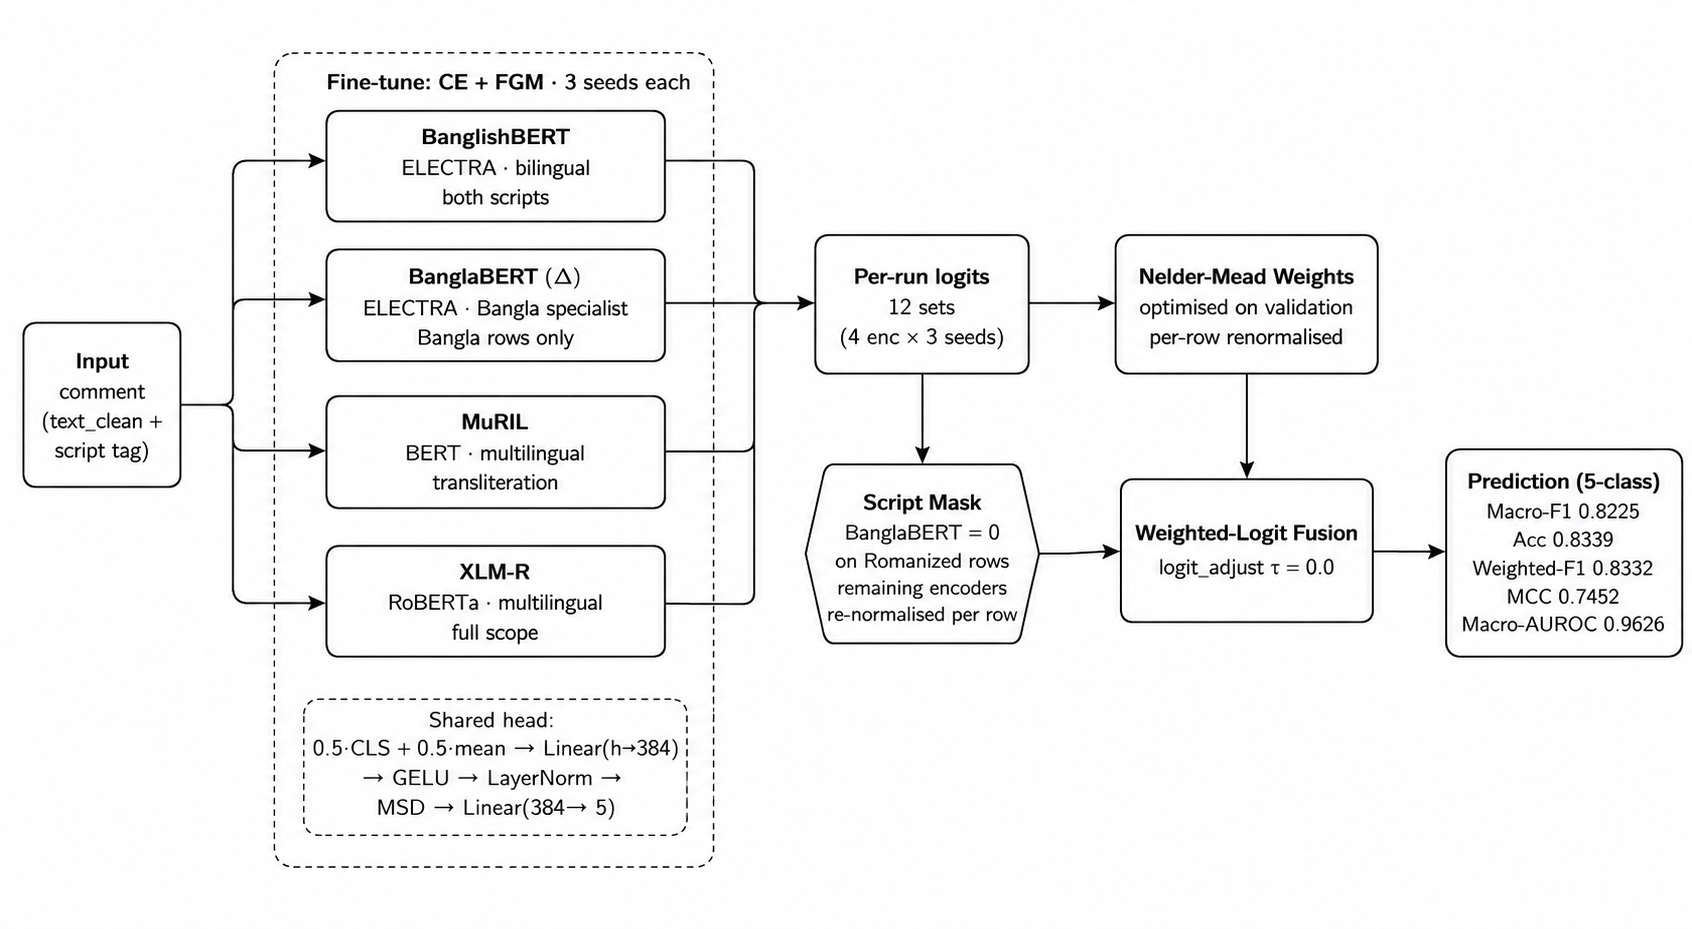
\includegraphics[width=1.0\textwidth]{D2_Script_Aware_Ensemble.png}
\caption{The proposed script-aware ensemble. A comment is routed by script. All four encoders process Bangla-script comments; on Romanized comments the Bangla-script specialist BanglaBERT emits neutral logits and receives zero fusion weight, so the remaining encoders decide the label. Each encoder is fine-tuned with cross-entropy plus FGM across three seeds, and the twelve resulting logit vectors are fused by validation-optimised weights.}
\label{fig:ensemble}
\end{figure}

\begin{table}[!htbp]
\centering
\caption{Notation used in \cref{sec:methodology}.}
\label{tab:notation}
\small
\begin{tabularx}{\textwidth}{@{}lX@{}}
\toprule
\textbf{Symbol} & \textbf{Meaning} \\
\midrule
$x$, $y$ & Input comment (token sequence) and its ground-truth class \\
$T$, $C$ & Sequence length ($\le 128$ tokens) and number of classes ($C = 5$) \\
$s(x) \in \{\textsc{bn}, \textsc{rom}\}$ & Script of comment $x$: Bangla or Romanized \\
$\mathbf{e} \in \mathbb{R}^{T \times d}$ & Input-embedding matrix (token $+$ position), $d = 768$ \\
$H$, $d_k$, $d_{\mathrm{ff}}$ & Attention heads, per-head width $d_k = d/H$, and FFN inner width ($3072$) \\
$\mathbf{W}^Q_i, \mathbf{W}^K_i, \mathbf{W}^V_i$ & Query, key, value projections of head $i$ \\
$\theta_m$, $\phi_m$ & Encoder and head parameters of backbone $m$ \\
$\mathbf{h}_t \in \mathbb{R}^{d}$ & Contextual hidden state at position $t$; $\mathbf{h}_{[\mathrm{CLS}]} \equiv \mathbf{h}_0$ \\
$\mathbf{z}_m \in \mathbb{R}^{C}$ & Logit vector from backbone $m$ \\
$\hat{p}(y \mid x) \in \Delta^{C-1}$ & Predicted class-probability vector \\
$\mathbf{r}$ & Embedding-space adversarial perturbation (FGM) \\
$\epsilon$ & FGM perturbation budget \\
$w_m \ge 0$ & Fusion weight of ensemble member $m$, $\sum_m w_m = 1$ \\
$\mathcal{M}$, $\mathcal{M}(x)$ & Full member set (12) and the active members for comment $x$ \\
\bottomrule
\end{tabularx}
\end{table}

\subsection{From a Comment to Contextual Embeddings}
\label{sec:prelim}

Take a single Romanized comment, $x = $ \emph{``tui akta faltu manush''} (roughly, \emph{``you are a worthless person''}). A backbone's subword tokeniser turns it into a sequence of $T$ token ids $(w_1,\ldots,w_T)$ with a leading \texttt{[CLS]} and trailing \texttt{[SEP]}. Each id is mapped to a $d$-dimensional vector by a token-embedding lookup $\mathbf{E}_{\mathrm{tok}} \in \mathbb{R}^{V \times d}$ and added to a position embedding, so the input row for position $t$ is
\begin{equation}
\mathbf{e}_t = \mathbf{E}_{\mathrm{tok}}[w_t] + \mathbf{E}_{\mathrm{pos}}[t], \qquad \mathbf{e} = (\mathbf{e}_1,\ldots,\mathbf{e}_T) \in \mathbb{R}^{T \times d},
\label{eq:embed}
\end{equation}
with $d = 768$. The encoder is a stack of $L = 12$ transformer blocks \citep{vaswani2017attention}. Each block first contextualises the sequence $\mathbf{H} \in \mathbb{R}^{T \times d}$ with multi-head self-attention. For head $i \in \{1,\ldots,H\}$ the block projects $\mathbf{H}$ into queries, keys, and values, then applies scaled dot-product attention,
\begin{equation}
\mathbf{Q}_i = \mathbf{H}\mathbf{W}^Q_i,\quad \mathbf{K}_i = \mathbf{H}\mathbf{W}^K_i,\quad \mathbf{V}_i = \mathbf{H}\mathbf{W}^V_i,
\qquad
\mathrm{head}_i = \mathrm{softmax}\!\left(\frac{\mathbf{Q}_i \mathbf{K}_i^{\top}}{\sqrt{d_k}} + \mathbf{M}\right)\mathbf{V}_i,
\label{eq:attention}
\end{equation}
where $\mathbf{W}^Q_i, \mathbf{W}^K_i, \mathbf{W}^V_i \in \mathbb{R}^{d \times d_k}$, $d_k = d/H$, and $\mathbf{M}$ is an additive mask sending padded positions to $-\infty$ so they receive zero attention weight. The row-wise softmax produces an attention matrix $\mathbf{A}_i \in \mathbb{R}^{T \times T}$ whose entry $A_{i,ts}$ is the weight token $t$ places on token $s$; this is the mechanism that binds \emph{faltu} (``worthless'') to \emph{manush} (``person''), since the insult lives in their pairing rather than either token alone. The $H$ heads are concatenated and mixed by an output projection $\mathbf{W}^O \in \mathbb{R}^{d \times d}$,
\begin{equation}
\mathrm{MHA}(\mathbf{H}) = \mathrm{Concat}(\mathrm{head}_1,\ldots,\mathrm{head}_H)\,\mathbf{W}^O .
\label{eq:mha}
\end{equation}
A position-wise feed-forward network then lifts each token to an inner width $d_{\mathrm{ff}} = 3072$ and back,
\begin{equation}
\mathrm{FFN}(\mathbf{x}) = \mathrm{GELU}(\mathbf{x}\mathbf{W}_1^{\mathrm{ff}} + \mathbf{b}_1^{\mathrm{ff}})\,\mathbf{W}_2^{\mathrm{ff}} + \mathbf{b}_2^{\mathrm{ff}},
\qquad \mathbf{W}_1^{\mathrm{ff}} \in \mathbb{R}^{d \times d_{\mathrm{ff}}},\ \mathbf{W}_2^{\mathrm{ff}} \in \mathbb{R}^{d_{\mathrm{ff}} \times d},
\label{eq:ffn}
\end{equation}
and each sub-layer is wrapped in a residual connection and layer normalisation,
\begin{equation}
\mathbf{H}' = \mathrm{LN}\!\big(\mathbf{H} + \mathrm{MHA}(\mathbf{H})\big),
\qquad
\mathbf{H}'' = \mathrm{LN}\!\big(\mathbf{H}' + \mathrm{FFN}(\mathbf{H}')\big),
\label{eq:block}
\end{equation}
where $\mathrm{LN}(\mathbf{x}) = \gamma \odot (\mathbf{x} - \mu)/\sqrt{\sigma^2 + \varepsilon} + \beta$ standardises each token vector over its $d$ features using the per-token mean $\mu$ and variance $\sigma^2$, with learned scale $\gamma$ and shift $\beta$. Stacking the twelve blocks on top of $\mathbf{e}$ yields contextual hidden states $(\mathbf{h}_0, \ldots, \mathbf{h}_{T-1})$, collecting the parameters of all blocks, embeddings, and projections into the encoder set $\theta_m$.

Two of our backbones, BanglaBERT and BanglishBERT \citep{bhattacharjee2022banglabert}, are pretrained as ELECTRA discriminators \citep{clark2020electra} rather than masked language models: a small generator replaces some tokens and the discriminator learns to flag which ones were replaced, an objective that yields strong Bengali representations from 27.5\,GB of text. MuRIL and XLM-R are standard masked-LM encoders. For our purposes the pretraining objective matters only through the representations it produces; the fine-tuning path below is identical across all four.

\subsection{Pooling and Classification Head}
\label{sec:head}

Each backbone $m$ carries the same lightweight head. We pool the sequence by blending the \texttt{[CLS]} vector with a mean over token states, which is steadier than \texttt{[CLS]} alone on short, noisy comments:
\begin{equation}
\mathbf{h}_{\mathrm{pool}} = \tfrac{1}{2}\,\mathbf{h}_{[\mathrm{CLS}]} + \tfrac{1}{2}\cdot\frac{\sum_{t=1}^{T} m_t\,\mathbf{h}_t}{\sum_{t=1}^{T} m_t},
\label{eq:pool}
\end{equation}
where $m_t \in \{0,1\}$ is the attention mask that zeroes out padding. The pooled vector passes through a small projection with GELU and LayerNorm, then a linear layer to $C$ logits:
\begin{equation}
\mathbf{u} = \mathrm{LN}\!\big(\mathrm{GELU}(\mathbf{W}_1 \mathbf{h}_{\mathrm{pool}} + \mathbf{b}_1)\big) \in \mathbb{R}^{384},
\qquad
\mathbf{z}_m = \mathbf{W}_2\,\mathbf{u} + \mathbf{b}_2 \in \mathbb{R}^{C},
\label{eq:head}
\end{equation}
with $\mathbf{W}_1 \in \mathbb{R}^{384 \times d}$ and $\mathbf{W}_2 \in \mathbb{R}^{C \times 384}$. The class probabilities are $\hat{p}(y \mid x) = \mathrm{softmax}(\mathbf{z}_m)$. For our example comment, a well-trained encoder puts most of the softmax mass on \emph{abusive}.

\subsection{Training Objective: Cross-Entropy with FGM}
\label{sec:objective}

Each backbone is fine-tuned end-to-end (both $\theta_m$ and $\phi_m$) with AdamW \citep{loshchilov2019adamw} under a mild label-smoothed cross-entropy. With smoothing $s = 0.03$ the soft target is $\tilde{y}_c = (1-s)\,\mathbb{1}[c = y] + s/C$, and
\begin{equation}
\mathcal{L}_{\mathrm{CE}}(\theta_m, \phi_m) = -\frac{1}{N}\sum_{i=1}^{N}\sum_{c=1}^{C} \tilde{y}_{i,c}\,\log \hat{p}(y = c \mid x_i).
\label{eq:ce}
\end{equation}
Cross-entropy alone leaves the decision boundary brittle in directions the training set does not cover, which for user-generated Bengali means small spelling changes can flip a prediction. Adversarial training addresses this by asking, for each batch, what small perturbation of the input embeddings would most increase the loss, and then training against it. Formally it is a min--max problem,
\begin{equation}
\min_{\theta_m, \phi_m}\; \mathbb{E}_{(x,y)}\Big[\max_{\|\mathbf{r}\|_2 \le \epsilon}\; \mathcal{L}_{\mathrm{CE}}\big(\mathbf{e}(x) + \mathbf{r},\, y\big)\Big].
\label{eq:minmax}
\end{equation}
FGM \citep{miyato2017adversarial} solves the inner maximisation in closed form to first order. Let $\mathbf{g} = \nabla_{\mathbf{e}}\mathcal{L}_{\mathrm{CE}}(\mathbf{e},y)$ be the gradient of the loss with respect to the input embeddings. A first-order Taylor expansion around $\mathbf{r} = \mathbf{0}$ gives $\mathcal{L}_{\mathrm{CE}}(\mathbf{e} + \mathbf{r}, y) \approx \mathcal{L}_{\mathrm{CE}}(\mathbf{e}, y) + \mathbf{r}^{\top}\mathbf{g}$, so the inner problem reduces to maximising the linear form $\mathbf{r}^{\top}\mathbf{g}$ subject to $\|\mathbf{r}\|_2 \le \epsilon$. By the Cauchy--Schwarz inequality this is maximised when $\mathbf{r}$ is parallel to $\mathbf{g}$ and saturates the norm constraint, which yields
\begin{equation}
\boxed{\;\mathbf{r}_{\mathrm{adv}} = \epsilon\,\frac{\mathbf{g}}{\|\mathbf{g}\|_2}\;}
\label{eq:fgm}
\end{equation}
a single ascent step on the embeddings scaled to the surface of the $\ell_2$-ball. Perturbing the continuous embeddings rather than the discrete token ids is what makes the attack differentiable and cheap: $\mathbf{g}$ is already available from the clean backward pass. The per-batch objective sums the clean and adversarial forward passes,
\begin{equation}
\mathcal{L}(\theta_m, \phi_m) = \mathcal{L}_{\mathrm{CE}}(\mathbf{e}, y) + \mathcal{L}_{\mathrm{CE}}(\mathbf{e} + \mathbf{r}_{\mathrm{adv}}, y),
\label{eq:fgm-loss}
\end{equation}
and both passes accumulate gradients into the same parameters before a single optimiser step (\cref{alg:fgm}). On \emph{``tui akta faltu manush''} the perturbation nudges the embeddings of \emph{faltu} and \emph{manush} in the loss-increasing direction, so training against it forces the decision to rest on the phrase's meaning rather than its exact spelling. FGM costs one extra forward--backward pass per batch and exposes a single hyperparameter $\epsilon$, fixed at $1.0$.

\paragraph{Parameter updates.} Both the encoder $\theta_m$ and the head $\phi_m$ are trained end to end. Writing $\Theta = (\theta_m, \phi_m)$ for all trainable parameters, the gradient from \cref{eq:fgm-loss} flows back through the head (\cref{eq:head,eq:pool}) and then through every transformer block (\cref{eq:block,eq:mha,eq:attention}) by the chain rule; for a single weight matrix $\mathbf{W}$ in block $\ell$ this is $\partial \mathcal{L}/\partial \mathbf{W} = \sum_t (\partial \mathcal{L}/\partial \mathbf{H}^{(\ell)}_t)(\partial \mathbf{H}^{(\ell)}_t/\partial \mathbf{W})$, with the attention softmax and GELU contributing their Jacobians along the path. The accumulated gradient $\mathbf{g}_\Theta = \nabla_\Theta \mathcal{L}$ drives an AdamW update \citep{loshchilov2019adamw}, which maintains bias-corrected first- and second-moment estimates $\hat{\mathbf{m}}_t, \hat{\mathbf{v}}_t$ and decouples weight decay from the gradient step,
\begin{align}
\mathbf{m}_t &= \beta_1 \mathbf{m}_{t-1} + (1-\beta_1)\,\mathbf{g}_\Theta, &
\mathbf{v}_t &= \beta_2 \mathbf{v}_{t-1} + (1-\beta_2)\,\mathbf{g}_\Theta^{2}, \label{eq:adam-moments}\\[2pt]
\hat{\mathbf{m}}_t &= \frac{\mathbf{m}_t}{1-\beta_1^{t}}, &
\hat{\mathbf{v}}_t &= \frac{\mathbf{v}_t}{1-\beta_2^{t}}, \nonumber\\[2pt]
\Theta_{t} &= \Theta_{t-1} - \eta\left(\frac{\hat{\mathbf{m}}_t}{\sqrt{\hat{\mathbf{v}}_t} + \varepsilon} + \lambda\,\Theta_{t-1}\right), \label{eq:adamw-update}
\end{align}
with $\beta_1 = 0.9$, $\beta_2 = 0.999$, decoupled weight decay $\lambda$, and a learning rate $\eta$ warmed up linearly and then decayed. The encoder and head use separate learning rates (\cref{tab:hparams}); gradients are clipped in $\ell_2$ norm before \cref{eq:adamw-update} to bound the step. Why FGM and nothing heavier is the subject of the ablation in \cref{sec:ablation-results}.

\begin{algorithm}[!htbp]
\caption{Cross-entropy $+$ FGM fine-tuning of one backbone (single mini-batch).}
\label{alg:fgm}
\begin{algorithmic}[1]
\Require Batch $(x, y)$, encoder $\theta_m$, head $\phi_m$, budget $\epsilon$
\State Embed: $\mathbf{e} \leftarrow \mathrm{Embed}(x)$
\State \textbf{Clean pass:} $\mathcal{L}_{\mathrm{clean}} \leftarrow \mathcal{L}_{\mathrm{CE}}(\mathbf{e}, y)$;\; \texttt{backward} (accumulate $\nabla_{\theta_m,\phi_m}$)
\State Compute $\mathbf{g} = \nabla_{\mathbf{e}}\mathcal{L}_{\mathrm{clean}}$;\; set $\mathbf{r}_{\mathrm{adv}} \leftarrow \epsilon\,\mathbf{g}/\|\mathbf{g}\|_2$ \Comment{\cref{eq:fgm}}
\State \textbf{FGM pass:} $\mathcal{L}_{\mathrm{adv}} \leftarrow \mathcal{L}_{\mathrm{CE}}(\mathbf{e} + \mathbf{r}_{\mathrm{adv}}, y)$;\; \texttt{backward} (accumulate);\; \textbf{restore} $\mathbf{e}$
\State \textbf{Optimiser step:} $\theta_m, \phi_m \leftarrow$ AdamW update (uniform LR, no decay)
\end{algorithmic}
\end{algorithm}

\subsection{Script-Aware Specialisation}
\label{sec:scriptaware}

The four backbones do not have equal competence on both scripts, and pretending they do wastes the strongest one. BanglaBERT is pretrained on Bangla-script text only; feeding it Romanized Bangla degrades its representations and, worse, drags the ensemble down on exactly the script it cannot read. We therefore make BanglaBERT a Bangla-script specialist. It trains, validates, and is evaluated only on Bangla-script rows. On a Romanized comment it emits a neutral zero logit vector and receives zero fusion weight, so it never votes on text it was not built for. BanglishBERT, pretrained bilingually, is the workhorse for Romanized input; MuRIL and XLM-R stay full-scope over both scripts. This gives the ensemble a clean specialist-plus-generalists structure: for a Bangla comment all four members are active, and for a Romanized comment the three script-capable members decide.

Concretely, define an activation indicator for member $m$ on comment $x$:
\begin{equation}
a_m(x) =
\begin{cases}
0 & \text{if } m \text{ is a BanglaBERT member and } s(x) = \textsc{rom},\\
1 & \text{otherwise.}
\end{cases}
\label{eq:activation}
\end{equation}
The active set is $\mathcal{M}(x) = \{\, m \in \mathcal{M} : a_m(x) = 1 \,\}$. For our Romanized example, the three BanglaBERT seed members drop out and the nine remaining members carry the decision.

\subsection{Weighted-Logit Fusion}
\label{sec:fusion}

The ensemble has $|\mathcal{M}| = 12$ members: four backbones, each fine-tuned under three seeds ($42, 123, 456$). Fusion is a script-masked weighted average of logits, renormalised per comment over the active members so that dropping BanglaBERT on Romanized rows does not shrink the total weight:
\begin{equation}
\mathbf{z}_{\mathrm{ens}}(x) = \sum_{m \in \mathcal{M}(x)} \frac{w_m}{\sum_{m' \in \mathcal{M}(x)} w_{m'}}\; \mathbf{z}_m(x),
\qquad
\hat{y}(x) = \arg\max_{c}\; \big[\mathbf{z}_{\mathrm{ens}}(x)\big]_c.
\label{eq:fusion}
\end{equation}
The weights are the solution of a constrained maximisation of validation Macro-F1 over the probability simplex,
\begin{equation}
\mathbf{w}^{\ast} = \arg\max_{\mathbf{w} \in \Delta^{11}} \; \mathrm{F1}_{\mathrm{macro}}^{\mathrm{val}}\!\big(\mathbf{w}\big),
\qquad
\Delta^{11} = \Big\{ \mathbf{w} \in \mathbb{R}^{12} : w_m \ge 0,\ \textstyle\sum_{m} w_m = 1 \Big\},
\label{eq:weightopt}
\end{equation}
where $\mathrm{F1}_{\mathrm{macro}}^{\mathrm{val}}(\mathbf{w})$ is the Macro-F1 obtained on the validation split when \cref{eq:fusion} is decoded with weights $\mathbf{w}$. This objective is piecewise constant in $\mathbf{w}$: its value changes only when some comment's argmax flips, so the gradient is zero almost everywhere and undefined at the flip boundaries. Gradient methods are therefore useless here, which is why we solve \cref{eq:weightopt} with the derivative-free Nelder--Mead simplex search \citep{nelder1965simplex}. The algorithm maintains a simplex of thirteen candidate weight vectors in $\mathbb{R}^{12}$ and, at each iteration, replaces the worst vertex using the standard reflection, expansion, contraction, and shrink moves (coefficients $\alpha = 1$, $\gamma = 2$, $\rho = \tfrac{1}{2}$, $\sigma = \tfrac{1}{2}$); candidates that leave the simplex are clipped at zero and renormalised, which projects them back onto $\Delta^{11}$. The search starts from the uniform vector $w_m = \tfrac{1}{12}$, so the optimiser has to earn any departure from plain averaging. Each objective evaluation is cheap because the twelve members' validation logits are computed once and cached; evaluating a candidate $\mathbf{w}$ is then a weighted sum, an argmax, and one Macro-F1 computation over the 9{,}432 validation rows, so the whole search costs seconds. The weights are fitted once, frozen before the 20\% test set is ever seen, and reported in \cref{sec:ensemble-results}, so the test numbers stay clean. An optional inference-time logit adjustment for the long tail \citep{menon2021longtail} is available but tuned to zero strength on this benchmark, so the fused logits above are the final decision.

\subsection{A Worked Example on Two Scripts}
\label{sec:worked-example}

Following one comment through the system in each script makes the routing concrete. \Cref{fig:worked} traces both cases end to end.

Take the Romanized comment $x_1 = $ \emph{``tui akta faltu manush''}. Its script is $s(x_1) = \textsc{rom}$, so \cref{eq:activation} switches the three BanglaBERT seed members off and $\mathcal{M}(x_1)$ holds nine members. The tokeniser produces \texttt{[CLS] tui akta fal \#\#tu manush [SEP]} and the embedding layer gives $\mathbf{e} \in \mathbb{R}^{T \times 768}$ (\cref{eq:embed,eq:attention}). Each active encoder pools through \cref{eq:pool,eq:head} into a logit vector; a representative one places its mass at roughly $[\text{ab } 0.61,\ \text{no } 0.20,\ \text{se } 0.11,\ \text{re } 0.04,\ \text{th } 0.04]$. FGM shaped that decision in training by perturbing the embeddings of \emph{faltu} and \emph{manush} along the loss gradient (\cref{eq:fgm}), so the model leans on the phrase rather than its spelling. Fusion renormalises the nine active weights and averages the logits (\cref{eq:fusion}); the argmax is \emph{abusive}.

For the Bangla-script comment $x_2 = $ \bn{তুই একটা বাজে লোক}{tui akta baje lok} (``you are a bad person''), $s(x_2) = \textsc{bn}$, every $a_m(x_2) = 1$, and all twelve members vote, the specialist included. Pooling, head, and fusion are unchanged and the argmax is again \emph{abusive}. The two traces differ in exactly one place, which members are active, and that single difference is the whole of the script-aware design.

\begin{figure}[!htbp]
\centering
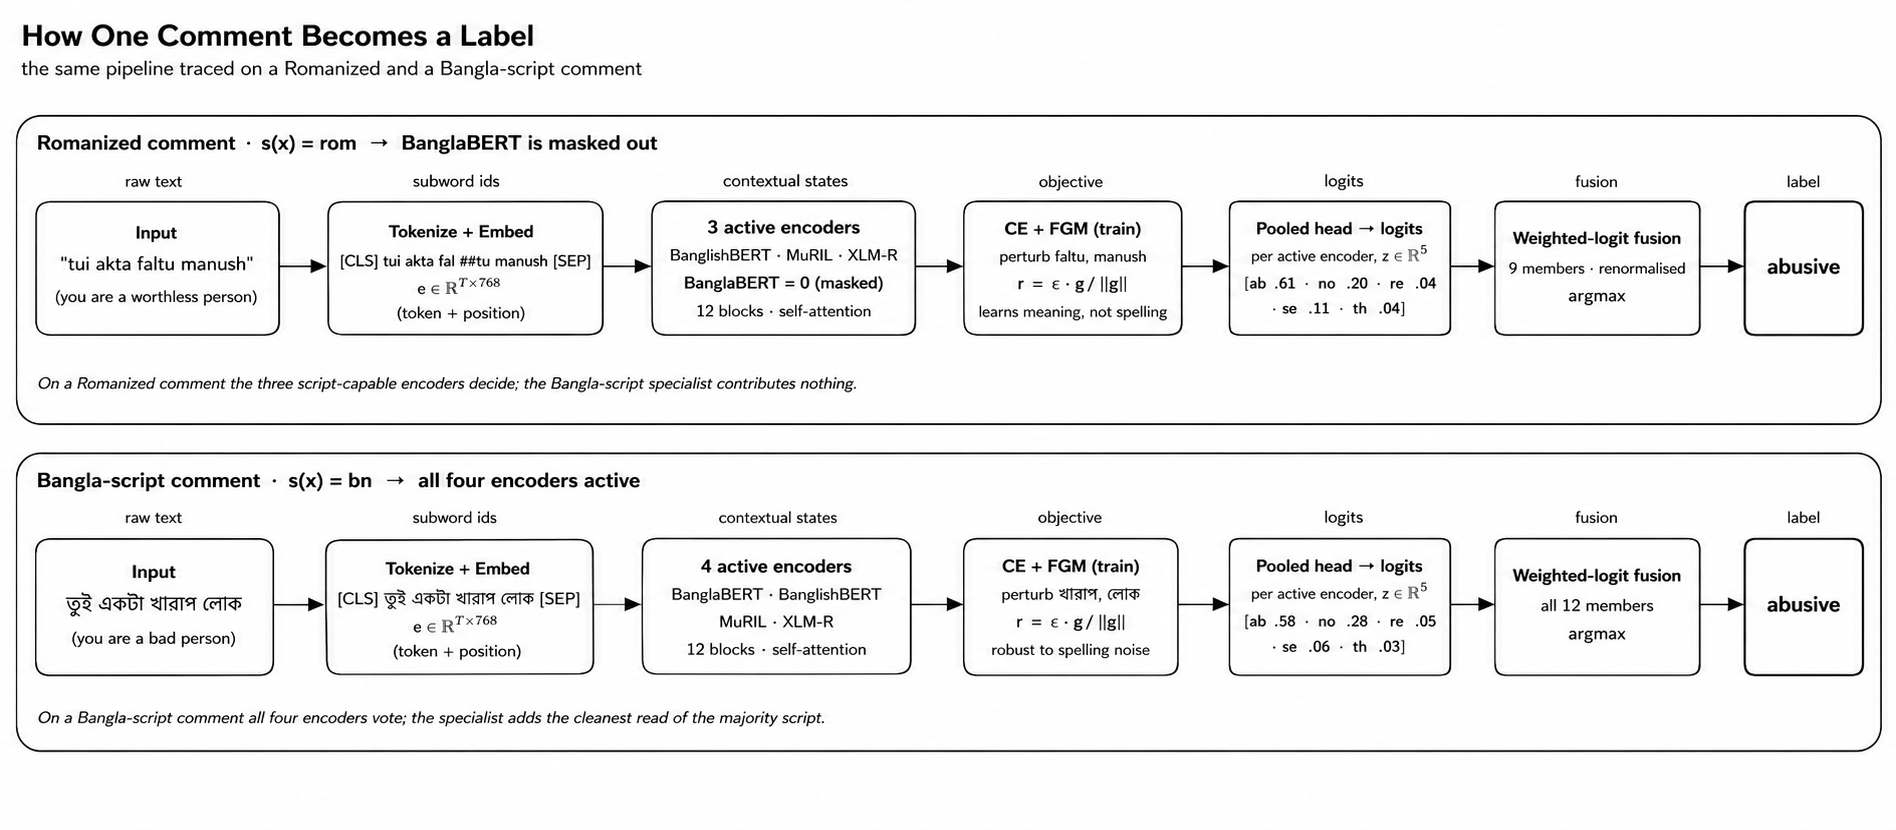
\includegraphics[width=0.99\textwidth]{D3_Worked_Example.png}
\caption{One comment traced through the system in each script. Top: a Romanized comment, where the Bangla-script specialist is masked out and nine members decide. Bottom: a Bangla-script comment, where all twelve members vote. Every other stage, tokenisation, embedding, encoding, the CE$+$FGM objective, pooling, and weighted-logit fusion, is identical across the two scripts.}
\label{fig:worked}
\end{figure}


% =============================================================
% SECTION 5 — EXPERIMENTAL SETUP
% =============================================================
\section{Experimental Setup}
\label{sec:setup}

\subsection{Backbones and Training Configuration}
\label{sec:config}

The four encoders are BanglishBERT (\texttt{csebuetnlp/\allowbreak banglishbert}, bilingual), BanglaBERT (\texttt{csebuetnlp/\allowbreak banglabert}, Bangla-script specialist), MuRIL (\texttt{google/\allowbreak muril-base-cased}), and XLM-R (\texttt{xlm-roberta-base}). All share the pooling and head of \cref{sec:head}. \Cref{tab:hparams} lists the training configuration, held fixed across backbones so that any difference between them reflects the encoder, not incidental tuning. Two choices are worth flagging. Learning rate is uniform with no decay, because an early experiment found that layer-wise decay hurt on this multi-source, dual-script mixture. And the effective batch size is held at 32 across hardware. All runs use fp16 mixed precision on a single NVIDIA A6000 (48\,GB) with 32\,GB system RAM; software is PyTorch \citep{paszke2019pytorch} with HuggingFace Transformers \citep{wolf2020transformers} and scikit-learn \citep{pedregosa2011scikit}. Seeds are fixed at $\{42, 123, 456\}$.

\begin{table}[!htbp]
\centering
\caption{Training configuration for the four backbones. Held constant across encoders.}
\label{tab:hparams}
\small
\begin{tabularx}{\textwidth}{@{}lcX@{}}
\toprule
\textbf{Hyperparameter} & \textbf{Value} & \textbf{Notes} \\
\midrule
Optimiser & AdamW & $\beta_1 = 0.9$, $\beta_2 = 0.999$ \\
Encoder / head learning rate & $2\times10^{-5}$ / $8\times10^{-5}$ & uniform across layers, no layer-wise decay \\
AdamW weight decay $\lambda$ & 0.01 & decoupled, \cref{eq:adamw-update}; excludes bias and LayerNorm \\
LR schedule & linear & 10\% warm-up, then linear decay \\
Gradient clipping & 1.0 & global $\ell_2$ norm \\
Model selection & best validation Macro-F1 & checkpoint restored before test \\
Max sequence length & 128 & covers nearly the whole length distribution \\
Batch size (effective) & 32 & physical 32 $\times$ accumulation 1 \\
Epochs & up to 8 & early stopping, patience 3 \\
Label smoothing & 0.03 & mild \\
Dropout / head hidden & 0.25 / 384 & --- \\
FGM budget $\epsilon$ & 1.0 & embedding-space perturbation \\
Precision & fp16 & A6000 48\,GB \\
Seeds & 42, 123, 456 & three per backbone \\
\bottomrule
\end{tabularx}
\end{table}

\subsection{Evaluation Metrics}
\label{sec:metrics}

The primary metric is Macro-F1, reported with Weighted-F1 alongside. For $C$ classes,
\begin{equation}
\mathrm{F1}(c) = \frac{2\,\mathrm{Prec}(c)\,\mathrm{Rec}(c)}{\mathrm{Prec}(c) + \mathrm{Rec}(c)},
\qquad
\text{Macro-F1} = \frac{1}{C}\sum_{c=1}^{C} \mathrm{F1}(c).
\label{eq:macrof1}
\end{equation}
Macro-F1 weights every class equally, so the rare \emph{threat} and \emph{religious} classes are not hidden by the dominant \emph{none} class; Weighted-F1, which weights by support, is reported for continuity with prior work. We also report Accuracy and the Matthews correlation coefficient \citep{matthews1975mcc}, which is informative under imbalance because it uses every cell of the confusion matrix $\mathbf{K} \in \mathbb{N}^{C \times C}$. In its multiclass form,
\begin{equation}
\mathrm{MCC} =
\frac{\sum_{c} K_{cc} \cdot N \;-\; \sum_{c} \hat{n}_c\, n_c}
{\sqrt{\big(N^2 - \sum_{c} \hat{n}_c^{\,2}\big)\big(N^2 - \sum_{c} n_c^{2}\big)}},
\label{eq:mcc}
\end{equation}
where $N$ is the number of test comments, $n_c = \sum_{j} K_{cj}$ the true count of class $c$, and $\hat{n}_c = \sum_{i} K_{ic}$ its predicted count; the coefficient is $1$ for perfect prediction, $0$ at chance level, and is not inflated by majority-class dominance the way accuracy is. Finally we report one-vs-rest Macro-AUROC, the mean over classes of the area under the ROC curve treating each class against the rest, which measures the quality of the model's ranking independently of any decision threshold.

\subsection{Statistical Reporting}
\label{sec:stats}

Because the 20\% test set is a single fixed sample, we quantify its uncertainty with a percentile bootstrap \citep{efron1979bootstrap}. For a metric $T$ we draw $B = 2{,}000$ resamples of the 18{,}865 test predictions with replacement, recompute $T$ on each, and report the interval between the 2.5th and 97.5th percentiles:
\begin{equation}
\mathrm{CI}_{95\%} = \big[\, \hat{T}^{(\lceil 0.025 B \rceil)},\; \hat{T}^{(\lceil 0.975 B \rceil)} \,\big].
\label{eq:bootstrap}
\end{equation}
The resampling seed is fixed at 42. We report interval estimates rather than paired significance tests against the classical baselines, since those baselines are reference points rather than the comparison of interest.

\subsection{Computational Cost}
\label{sec:cost}

The whole system fits on a single 48\,GB GPU, which matters in a low-resource setting where clusters are not a given. Each backbone carries 110--135M parameters, so the twelve fine-tuning runs are the cost, not the fusion: the Nelder--Mead search runs over twelve scalars on cached validation logits and takes seconds. On the A6000 a backbone fine-tunes in 35--50 minutes at length 128 and batch 32, so the full ensemble reproduces in a few GPU-hours. FGM doubles a run's per-batch backward cost, but only in training; at inference the model is twelve forward passes (nine on Romanized input) plus a weighted average. We do not call the system lightweight. Twelve encoders is a committee, and a deployment that cannot afford one has a fallback in our own tables: the strongest full-scope single model (MuRIL, seed 123) reaches 0.8084 Macro-F1 on the same split (\cref{tab:perrun}), giving up $0.0141$ for a twelvefold cut in inference cost. That fallback must be full-scope, since the Bangla-script specialist abstains on Romanized input by design. Distilling the committee into one student is the natural production path and is left to future work.

\subsection{Component Ablation Design}
\label{sec:ablation-design}

The proposed recipe fine-tunes with cross-entropy plus FGM. Whether either piece earns its place, and whether anything beyond the pair does, is the question the ablation settles rather than assumes. We anchor on BanglishBERT and take plain cross-entropy as the reference. From there we add one component at a time, first FGM, then each of the standard imbalance and regularisation tools that the usual playbook stacks on top, and measure the change in Macro-F1. Every configuration is run over three seeds, so each number is a mean with a standard deviation and the small deltas can be judged against seed noise instead of at face value (\cref{sec:ablation-results}). The candidate components are defined here so their contributions are interpretable.

\emph{Class-balanced focal loss.} Focal loss \citep{lin2017focal} down-weights easy, confident examples so the optimiser attends to hard ones, and class-balanced weighting \citep{cui2019classbalanced} scales each class by the inverse of its effective sample count. With focusing parameter $\gamma$ and per-class weight $\alpha_c$,
\begin{equation}
\mathcal{L}_{\mathrm{focal}} = -\frac{1}{N}\sum_{i=1}^{N} \alpha_{y_i}\,\big(1 - \hat{p}_{i,y_i}\big)^{\gamma}\,\log \hat{p}_{i,y_i},
\qquad
\alpha_c \propto \frac{1 - \beta}{1 - \beta^{n_c}},
\label{eq:focal}
\end{equation}
where $n_c$ is the count of class $c$ and $\beta \to 1$ recovers inverse-frequency weighting. We use $\gamma = 2$ and $\beta = 0.999$.

\emph{Balanced sampler.} Instead of reweighting the loss, this reshapes the batch: each example is sampled with probability proportional to $n_{y_i}^{-1/2}$ (square-root inverse frequency), so minority classes appear more often during training.

\emph{Multi-sample dropout.} The head is evaluated under $K$ independent dropout masks and the losses are averaged, which reduces the variance of the head update at no inference cost \citep{inoue2019multisample}:
\begin{equation}
\mathcal{L}_{\mathrm{MSD}} = \frac{1}{K}\sum_{k=1}^{K} \mathcal{L}_{\mathrm{CE}}\!\big(\mathrm{head}(\mathrm{dropout}_k(\mathbf{h}_{\mathrm{pool}}))\big).
\label{eq:msd}
\end{equation}

\emph{R-Drop.} Two independent dropout passes over the same input give two distributions $\hat{p}^{(1)}, \hat{p}^{(2)}$; R-Drop \citep{liang2021rdrop} adds their symmetric KL divergence to the loss, pushing the two passes to agree and so regularising against dropout noise:
\begin{equation}
\mathcal{L}_{\mathrm{RDrop}} = \mathcal{L}_{\mathrm{CE}} + \frac{\lambda}{2}\Big[\mathrm{KL}\big(\hat{p}^{(1)} \,\|\, \hat{p}^{(2)}\big) + \mathrm{KL}\big(\hat{p}^{(2)} \,\|\, \hat{p}^{(1)}\big)\Big],
\label{eq:rdrop}
\end{equation}
with $\lambda = 0.5$.

\emph{Exponential moving average (EMA).} A shadow copy of the weights is maintained as an exponential moving average, $\bar{\theta} \leftarrow \mu\,\bar{\theta} + (1-\mu)\,\theta$ with $\mu = 0.999$, and used for evaluation. It is kept only when it beats the raw weights on validation, so it can never hurt.

Each component is a configuration toggle, which makes the ablation a direct read on what earns its place. The full-stack configuration turns all of them on at once.


% =============================================================
% SECTION 6 — RESULTS
% =============================================================
\section{Results and Analysis}
\label{sec:results}

We report in-domain benchmark results with bootstrap confidence intervals (\cref{sec:main-results}), a zero-shot LLM reference (\cref{sec:llm-baseline}), a per-class and error breakdown (\cref{sec:perclass-results}), the ablations that fix the training recipe and taxonomy (\cref{sec:ablation-results}), the effect of the script mask on Romanized-script Macro-F1 (\cref{sec:scriptmask-results}), cross-source robustness (\cref{sec:robustness-results}), the same-protocol comparison against the base paper (\cref{sec:basepaper-results}), and the learned ensemble weights (\cref{sec:ensemble-results}).

\subsection{In-Domain Benchmark}
\label{sec:main-results}

On the official 20\% test split ($n = 18{,}865$) the proposed model reaches Macro-F1 0.8225, Weighted-F1 0.8332, Accuracy 0.8339, MCC 0.7452, and Macro-AUROC 0.9626 (\cref{tab:main}). The strongest non-transformer reference, a word$+$character TF-IDF linear SVM, reaches 0.7674 Macro-F1; the proposed model is 5.5 Macro-F1 points above it. The gap is not a measurement artefact: the bootstrap 95\% intervals (\cref{tab:ci}) place Macro-F1 in $[0.8151, 0.8298]$, whose lower bound sits well clear of the reference's point estimate, and the same holds for every headline metric. \Cref{fig:main} shows the comparison, and \cref{fig:ci} shows the intervals.

\begin{table}[!htbp]
\centering
\caption{Main results on the official 20\% in-domain test split ($n = 18{,}865$). The reference is the strongest non-transformer baseline (TF-IDF word$+$char linear SVM).}
\label{tab:main}
\small
\begin{tabular}{@{}lccccc@{}}
\toprule
\textbf{System} & \textbf{Macro-F1} & \textbf{Weighted-F1} & \textbf{Accuracy} & \textbf{MCC} & \textbf{Macro-AUROC} \\
\midrule
Best non-transformer baseline & 0.7674 & 0.7889 & 0.7933 & 0.6788 & 0.9418 \\
\textbf{Proposed model} & \textbf{0.8225} & \textbf{0.8332} & \textbf{0.8339} & \textbf{0.7452} & \textbf{0.9626} \\
\bottomrule
\end{tabular}
\end{table}

\begin{table}[!htbp]
\centering
\caption{Bootstrap 95\% confidence intervals for the proposed model on the 20\% test split ($B = 2{,}000$, seed 42). Widths are computed from the rounded endpoints shown.}
\label{tab:ci}
\small
\begin{tabular}{@{}lccc@{}}
\toprule
\textbf{Metric} & \textbf{Value} & \textbf{95\% CI} & \textbf{CI width} \\
\midrule
Macro-F1 & 0.8225 & $[0.8151,\ 0.8298]$ & 0.0147 \\
Weighted-F1 & 0.8332 & $[0.8277,\ 0.8384]$ & 0.0107 \\
Accuracy & 0.8339 & $[0.8285,\ 0.8392]$ & 0.0107 \\
MCC & 0.7452 & $[0.7369,\ 0.7530]$ & 0.0161 \\
\bottomrule
\end{tabular}
\end{table}

\begin{figure}[!htbp]
\centering
\begin{subfigure}{0.49\textwidth}
\centering

\includegraphics[width=\textwidth]{fig02_main_results.png}
\caption{Proposed model vs.\ strongest baseline.}
\label{fig:main}
\end{subfigure}\hfill
\begin{subfigure}{0.49\textwidth}
\centering

\includegraphics[width=\textwidth]{fig11_bootstrap_ci.png}
\caption{Headline metrics with bootstrap 95\% CIs.}
\label{fig:ci}
\end{subfigure}
\caption{In-domain test performance. The proposed model clears the strongest non-transformer baseline on every metric, and the bootstrap intervals are narrow (Macro-F1 width 0.0147).}
\label{fig:main-combined}
\end{figure}

Per-backbone single-model scores (\cref{tab:perrun}) double as the transformer baseline suite: each row is a standard pretrained encoder fine-tuned with the identical recipe, so the table sits alongside the classical reference in \cref{tab:main}. The table spans two evaluation scopes and keeps them apart. BanglishBERT, MuRIL, and XLM-R are full-scope models scored on the complete test split; their best single run is MuRIL at 0.8084, with BanglishBERT (0.8083) and XLM-R (0.8052) just behind, so the three are close but not interchangeable. BanglaBERT is the Bangla-script specialist and by construction never predicts on Romanized text, so its rows are scored on the Bangla-script subset alone; its 0.8154 there says it reads the majority script cleanly, but it is a different measurement and cannot be lined up against the full-scope rows. The comparison that matters for the ensemble is therefore against the best full-scope member: the fused model reaches 0.8225 against MuRIL's 0.8084, a gain of $+0.0141$. That the committee clears its strongest directly comparable member by more than fourteen thousandths, while no single encoder dominates the others, is what tells us the fusion is exploiting genuine disagreement between the encoders rather than averaging away seed noise.

\begin{table}[!htbp]
\centering
\caption{Per-backbone, per-seed single-run scores, each a transformer baseline trained with the identical recipe. BanglishBERT, MuRIL, and XLM-R are full-scope and are scored on the complete 20\% test split ($n = 18{,}865$). BanglaBERT is the Bangla-script specialist of \cref{sec:scriptaware}: it never sees Romanized text in training or inference, so its rows are scored on the Bangla-script test subset only and are not directly comparable to the full-scope rows.}
\label{tab:perrun}
\small
\begin{tabular}{@{}llccccc@{}}
\toprule
\textbf{Backbone} & \textbf{Seed} & \textbf{Macro-F1} & \textbf{Weighted-F1} & \textbf{Accuracy} & \textbf{MCC} & \textbf{AUROC} \\
\midrule
BanglishBERT & 42 & 0.8069 & 0.8201 & 0.8206 & 0.7252 & 0.9567 \\
BanglishBERT & 123 & 0.7996 & 0.8124 & 0.8161 & 0.7151 & 0.9547 \\
BanglishBERT & 456 & 0.8083 & 0.8200 & 0.8213 & 0.7261 & 0.9568 \\
BanglaBERT$^{\dagger}$ & 42 & 0.8105 & 0.8178 & 0.8177 & 0.7545 & 0.9602 \\
BanglaBERT$^{\dagger}$ & 123 & 0.8154 & 0.8211 & 0.8218 & 0.7603 & 0.9599 \\
BanglaBERT$^{\dagger}$ & 456 & 0.8149 & 0.8205 & 0.8216 & 0.7600 & 0.9615 \\
MuRIL & 42 & 0.8055 & 0.8177 & 0.8185 & 0.7231 & 0.9521 \\
MuRIL & 123 & \textbf{0.8084} & 0.8216 & 0.8222 & \textbf{0.7284} & 0.9502 \\
MuRIL & 456 & 0.8066 & 0.8198 & 0.8210 & 0.7259 & 0.9523 \\
XLM-R & 42 & 0.8052 & 0.8159 & 0.8161 & 0.7199 & 0.9538 \\
XLM-R & 123 & 0.8016 & 0.8144 & 0.8145 & 0.7166 & 0.9503 \\
XLM-R & 456 & 0.8035 & 0.8173 & 0.8181 & 0.7215 & 0.9501 \\
\bottomrule
\end{tabular}

\vspace{2pt}
{\footnotesize $^{\dagger}$Bangla-script specialist: trained and evaluated on Bangla-script rows only, so these
scores are over the Bangla-script test subset and are not comparable with the full-scope rows above.
Bold marks the best full-scope run.}
\end{table}

\subsection{Zero-Shot LLM Reference}
\label{sec:llm-baseline}

It is worth asking whether the supervised pipeline is needed at all, since a strong instruction-tuned model can classify text from a prompt with no task-specific training. We tested it. We prompted Gemini 2.5 Flash~\citep{google2024gemini} (model identifier \texttt{google/gemini-2.5-flash}, accessed through the OpenRouter API in July 2026) with the same five-class definitions and priority rule the annotators used, and had it label every one of the 18{,}865 test comments zero-shot: one comment per request, temperature $0$, an output cap of eight tokens, and an instruction to emit the bare label word. Replies were matched against the five class names; a reply that matched none of them fell back to \emph{none}, the majority class, which is the conservative choice for a baseline. Failed requests were retried with exponential back-off. We scored the parsed output against the consolidated labels. Table~\ref{tab:llm} sets the result beside the proposed model on the same test split.

\begin{table}[!htbp]
\centering
\caption{Zero-shot large-language-model reference against the proposed supervised model, on the full 20\% test split ($n = 18{,}865$).}
\label{tab:llm}
\small
\begin{tabular}{@{}lcccc@{}}
\toprule
\textbf{System} & \textbf{Macro-F1} & \textbf{Weighted-F1} & \textbf{Accuracy} & \textbf{MCC} \\
\midrule
Gemini 2.5 Flash (zero-shot) & 0.5597 & 0.6684 & 0.6647 & 0.4957 \\
\textbf{Proposed model (supervised)} & \textbf{0.8225} & \textbf{0.8332} & \textbf{0.8339} & \textbf{0.7452} \\
\bottomrule
\end{tabular}
\end{table}

The gap is 26.3 Macro-F1 points in the proposed model's favour. The reason is partly the taxonomy and partly the script. A zero-shot model has no calibration for the intent-level line between generic abuse and clean speech, or for the culturally specific reading of religious and sexual harassment in Bengali, so it falls back on over-predicting the majority and the safe classes. It also meets a corpus that is 39.6\% Romanized Bangla, a low-resource surface form that general models handle unevenly. We treat this as a single-prompt zero-shot reference rather than a full evaluation of LLM-based moderation: a different prompt, a reasoning configuration, or a few in-context examples would all move the number, and we did not sweep them. What it does establish is a reference point, a benchmark-tuned committee of encoders clears a strong general model by 26 Macro-F1 points when that model is prompted directly, which is the practical case for releasing labelled Bengali data and a fitted system rather than leaning on an off-the-shelf LLM.

\subsection{Per-Class Performance and Error Analysis}
\label{sec:perclass-results}

The per-class picture (\cref{tab:perclass}) is where the taxonomy's difficulty shows. \emph{Religious} and \emph{none} are the strongest classes (F1 0.9031 and 0.8771), which makes sense: religious abuse carries distinctive vocabulary, and \emph{none} has by far the most training data. \emph{Sexual} follows at 0.8238. The two hard classes are \emph{threat} (0.7689) and \emph{abusive} (0.7397). \emph{Threat} is hard because it is rare (638 test items) and its bootstrap interval is correspondingly the widest, $[0.7429, 0.7951]$. \emph{Abusive} is hard for a different reason: it is the catch-all bucket, absorbing troll, personal, political, and spam behaviour, so its boundary with \emph{none} is genuinely fuzzy rather than under-sampled.

\begin{table}[!htbp]
\centering
\caption{Per-class precision, recall, F1, and bootstrap 95\% CI on the 20\% test split. Support is the number of test comments in each class.}
\label{tab:perclass}
\small
\begin{tabular}{@{}lccccr@{}}
\toprule
\textbf{Class} & \textbf{Precision} & \textbf{Recall} & \textbf{F1} & \textbf{95\% CI (F1)} & \textbf{Support} \\
\midrule
Religious & 0.9221 & 0.8848 & 0.9031 & $[0.8924,\ 0.9143]$ & 1{,}606 \\
None & 0.8622 & 0.8925 & 0.8771 & $[0.8719,\ 0.8819]$ & 9{,}463 \\
Sexual & 0.8359 & 0.8120 & 0.8238 & $[0.8107,\ 0.8356]$ & 2{,}165 \\
Threat & 0.7878 & 0.7508 & 0.7689 & $[0.7429,\ 0.7951]$ & 638 \\
Abusive & 0.7532 & 0.7266 & 0.7397 & $[0.7301,\ 0.7486]$ & 4{,}993 \\
\midrule
\textbf{Macro avg.} & 0.8322 & 0.8133 & 0.8225 & $[0.8151,\ 0.8298]$ & 18{,}865 \\
\bottomrule
\end{tabular}
\end{table}

The confusion matrix (\cref{fig:confusion}) confirms where the errors live. The largest off-diagonal mass is the \emph{abusive}$\leftrightarrow$\emph{none} pair: 1{,}081 true-\emph{abusive} comments predicted \emph{none} and 856 true-\emph{none} predicted \emph{abusive}. This is the same semantic-overlap problem the base paper reports between its Troll and Not-Bully classes, and it is intrinsic to the task: mild or sarcastic abuse and blunt-but-clean speech are separated by intent that the surface text does not always carry. The next-largest confusions (\cref{fig:topconf}) are \emph{sexual}$\to$\emph{abusive} (225) and \emph{abusive}$\to$\emph{sexual} (195), again a content-overlap pair. \emph{Threat}, despite being smallest, keeps 479 of its items on the diagonal, so the model is not simply abandoning the rare class.

\begin{figure}[!htbp]
\centering
\begin{subfigure}{0.52\textwidth}
\centering

\includegraphics[width=\textwidth]{fig04_confusion_matrix.png}
\caption{Counts.}
\label{fig:confusion}
\end{subfigure}\hfill
\begin{subfigure}{0.46\textwidth}
\centering

\includegraphics[width=\textwidth]{fig05_top_confusions.png}
\caption{Largest off-diagonal error pairs.}
\label{fig:topconf}
\end{subfigure}
\caption{Confusion structure of the proposed model on the 20\% test split. Errors concentrate on the \emph{abusive}$\leftrightarrow$\emph{none} boundary, an intent-level overlap rather than a data-scarcity problem.}
\label{fig:confusion-combined}
\end{figure}

Reading the misclassified comments shows three recurring, explainable patterns rather than random noise (\cref{tab:errorpatterns}). The first is intent ambiguity on the \emph{abusive}--\emph{none} boundary: sarcasm, reclaimed slurs among friends, and blunt-but-clean criticism all sit where the surface text does not disambiguate, and this is where the bulk of the 1{,}081 and 856 cross-errors fall. The second is content overlap between \emph{sexual} and \emph{abusive}: a comment can be both misogynistic and generically abusive, and a single-label taxonomy forces one choice. The third is minority dilution for \emph{threat}: implicit threats without violent keywords lean toward \emph{abusive}, which is why \emph{threat} recall (0.75) trails its precision (0.79). Most of this reflects genuine boundary ambiguity, which is why the model plateaus where it does rather than at a ceiling set by data volume; separating true semantic ambiguity from residual label noise across the four annotation teams would need a dedicated audit beyond the validation study of \cref{sec:taxonomy}.

\begin{table}[!htbp]
\centering
\caption{The three recurring error patterns behind the largest off-diagonal cells, with the mechanism and the count of test comments each accounts for.}
\label{tab:errorpatterns}
\small
\begin{tabularx}{\textwidth}{@{}l>{\raggedright\arraybackslash}Xr@{}}
\toprule
\textbf{Error pattern} & \textbf{Mechanism} & \textbf{Count} \\
\midrule
Abusive $\leftrightarrow$ None & Intent ambiguity: sarcasm, in-group language, and blunt-but-clean criticism are not separable from the surface text alone. & 1{,}937 \\
Sexual $\leftrightarrow$ Abusive & Content overlap: misogynistic comments are also generically abusive, and the single-label scheme forces one class. & 420 \\
Threat $\to$ Abusive & Minority dilution: implicit threats without violent keywords drift into the larger \emph{abusive} bucket. & 48 \\
\bottomrule
\end{tabularx}
\end{table}

\subsection{Ablations}
\label{sec:ablation-results}

\paragraph{Component ablation.} \Cref{tab:component} builds the recipe up from plain cross-entropy, one component at a time, three seeds each. The first addition is the decisive one: FGM lifts Macro-F1 from $0.7961$ to $0.8071$, a gain of $+0.0110$ that is roughly five times the seed-to-seed standard deviation of the cross-entropy reference ($0.0022$) and comes with the tightest spread of any configuration ($\pm0.0009$). Adversarial perturbation of the embeddings is the most valuable ingredient after the encoder itself, matching the intuition of \cref{sec:objective}: user-generated Bengali varies wildly at the surface, and training against worst-case embedding perturbations buys tolerance to that variation.

Everything after FGM is second-order. EMA ($+0.0022$ over FGM, $\pm0.0004$) and R-Drop ($+0.0012$, $\pm0.0006$) each add a small gain whose error bars clear the FGM baseline; MSD is flat ($-0.0003$) and focal-plus-class-weighting slightly trails ($-0.0016$). Two configurations move the number clearly the wrong way: the balanced sampler drops to $0.7995$ with the widest spread ($\pm0.0026$), and the full stack falls to $0.8042$, below five of the seven simpler recipes. Both regress for the same reason, over-correction: reweighting the batch distribution and piling consistency and averaging penalties on one another distort the objective more than the residual imbalance they target. The proposed model therefore stops at CE$+$FGM. This is a parsimony choice rather than the top of the table: EMA and R-Drop would each add one to two thousandths per backbone, but the twelve-member ensemble already averages three seeds per encoder, delivering the variance reduction those components target, and CE$+$FGM keeps the recipe at a single tunable hyperparameter. \Cref{fig:ablation} plots the trajectory.

\begin{table}[!htbp]
\centering
\caption{Component ablation on the imbalanced 20\% test split, anchored on BanglishBERT, three seeds per configuration (mean $\pm$ std). The reference is plain cross-entropy; each row adds one component. $\Delta_{\mathrm{CE}}$ is the change in mean Macro-F1 relative to the cross-entropy reference. FGM is the only large, tight gain; the balanced sampler and the full stack regress.}
\label{tab:component}
\small
\begin{tabular}{@{}lcccccr@{}}
\toprule
\textbf{Configuration} & \textbf{Macro-F1} & \textbf{Weighted-F1} & \textbf{Accuracy} & \textbf{MCC} & \textbf{AUROC} & \textbf{$\Delta_{\mathrm{CE}}$} \\
\midrule
CE only (reference) & $0.7961 \pm 0.0022$ & 0.8087 & 0.8093 & 0.7079 & 0.9470 & $+0.0000$ \\
$+$ FGM & $0.8071 \pm 0.0009$ & 0.8199 & 0.8218 & 0.7262 & 0.9557 & $+0.0110$ \\
$+$ focal $+$ class weights & $0.8055 \pm 0.0012$ & 0.8178 & 0.8197 & 0.7232 & 0.9553 & $+0.0094$ \\
$+$ balanced sampler & $0.7995 \pm 0.0026$ & 0.8115 & 0.8114 & 0.7129 & 0.9428 & $+0.0034$ \\
$+$ multi-sample dropout & $0.8068 \pm 0.0014$ & 0.8187 & 0.8207 & 0.7248 & 0.9564 & $+0.0107$ \\
$+$ R-Drop & $0.8083 \pm 0.0006$ & 0.8206 & 0.8231 & 0.7280 & 0.9568 & $+0.0123$ \\
$+$ EMA & $\mathbf{0.8093 \pm 0.0004}$ & 0.8212 & 0.8220 & 0.7273 & 0.9576 & $+0.0132$ \\
Full stack (all on) & $0.8042 \pm 0.0019$ & 0.8145 & 0.8143 & 0.7176 & 0.9529 & $+0.0081$ \\
\bottomrule
\end{tabular}
\end{table}

\begin{figure}[!htbp]
\centering

\includegraphics[width=0.82\textwidth]{fig06_component_ablation.png}
\caption{Component ablation, mean $\pm$ std over three seeds. FGM is the decisive gain over the cross-entropy reference (dashed); EMA and R-Drop add small further improvements, while the balanced sampler and the full stack fall back. The proposed model fine-tunes each backbone with CE$+$FGM.}
\label{fig:ablation}
\end{figure}

\paragraph{Taxonomy ablation.} Splitting the five classes into nine (adding \texttt{personal, political, gender, other}) collapses Macro-F1 from 0.8073 to 0.6140 under the same CE$+$FGM recipe (\cref{tab:taxonomy}, \cref{fig:taxonomy}). Weighted-F1 barely moves (0.8203 $\to$ 0.8020) because the majority classes are untouched; the Macro-F1 crash is entirely the four new classes, each of which is too sparse to learn from. This is the empirical case for the five-class headline: the finer taxonomy is not learnable at this data scale, and reporting Weighted-F1 alone would have hidden the collapse behind an almost unchanged number.

\begin{table}[!htbp]
\centering
\caption{Taxonomy ablation under the same recipe. The finer nine-class scheme crashes Macro-F1 while leaving Weighted-F1 nearly unchanged, exposing unlearnable rare classes.}
\label{tab:taxonomy}
\small
\begin{tabular}{@{}lccccc@{}}
\toprule
\textbf{Taxonomy} & \textbf{Macro-F1} & \textbf{Weighted-F1} & \textbf{Accuracy} & \textbf{MCC} & \textbf{AUROC} \\
\midrule
5-class (headline) & \textbf{0.8073} & 0.8203 & 0.8214 & 0.7255 & 0.9556 \\
9-class (ablation) & 0.6140 & 0.8020 & 0.8069 & 0.7071 & 0.9460 \\
\bottomrule
\end{tabular}
\end{table}

\begin{figure}[!htbp]
\centering

\includegraphics[width=0.52\textwidth]{fig07_taxonomy_ablation.png}
\caption{Taxonomy ablation. Macro-F1 drops from 0.807 to 0.614 when the task expands from five to nine classes, driven entirely by the sparse added classes.}
\label{fig:taxonomy}
\end{figure}

\subsection{The Script Mask and Romanized-Script Macro-F1}
\label{sec:scriptmask-results}

The ``script-aware'' design rests on one decision: masking the Bangla-script specialist off Romanized comments (\cref{sec:scriptaware}). That decision is testable directly, by comparing the proposed masked ensemble against an otherwise identical ensemble in which every backbone, BanglaBERT included, votes on every comment. \cref{tab:scriptmask} reports Macro-F1 on the Romanized subset, where the mask acts.

\begin{table}[!htbp]
\centering
\caption{Effect of the script mask on Romanized-script Macro-F1. Masking the Bangla-script specialist (BanglaBERT) off Romanized comments is compared against letting every backbone vote on every comment.}
\label{tab:scriptmask}
\small
\begin{tabular}{@{}lc@{}}
\toprule
\textbf{Setting} & \textbf{Romanized Macro-F1} \\
\midrule
No script mask (all backbones vote) & 0.4568 \\
Script-aware mask (proposed) & \textbf{0.4774} \\
\bottomrule
\end{tabular}
\end{table}

Two things are visible here. First, the absolute Romanized Macro-F1 sits in the mid-$0.4$ range in both settings, and that is a property of the data rather than of the mask. Romanized Bangla is the minority script (39.6\% of the corpus) and its rare classes are rarer still, so the per-class support Macro-F1 averages over is thin; it also has no spelling standard and heavy code-mixing, which makes it intrinsically the harder script (\cref{sec:rw-script}). The mid-$0.4$ ceiling is the difficulty of a hard, data-poor slice rather than a shortfall introduced by the model, and closing it is chiefly a matter of Romanized data volume.

Second, and this is what the mask exists for, specialising BanglaBERT lifts Romanized Macro-F1 by $+0.0206$ (from $0.4568$ to $0.4774$). Pretrained on Bangla script alone, BanglaBERT contributes noisy predictions on Latin-script text that drag the committee down when it is allowed to vote there; silencing it lets the three script-capable encoders decide and the Romanized number rises. The mask is a working part of the model's competence on Romanized Bangla, so the ``script-aware'' label rests on a measured effect and not on design intuition (\cref{sec:limitations}).

\subsection{Cross-Source Robustness}
\label{sec:robustness-results}

Random-split accuracy answers whether the model generalises to unseen comments from the same mixture. The question a deployment faces is harder: does it generalise to an unseen \emph{source}? We answer it with the three interpretable source-shift configurations from \cref{sec:splits}, holding each Bangla-script source out in turn, training on the rest, and testing on the held-out one, with the \texttt{uid} assertion guaranteeing no leakage. (The \dset{banth} hold-out is excluded by the scoping argument given there: it compounds source and script shift, so its number would measure neither cleanly.) \cref{tab:robustness} reports the three configurations, and \cref{fig:robustness} plots them against the in-domain line.

\begin{table}[!htbp]
\centering
\caption{Source-held-out robustness of the proposed model, three Bangla-script sources, four encoders, three seeds per configuration (mean $\pm$ std on Macro-F1). Each row trains on the other two Bangla-script sources and tests on the full held-out source. The in-domain reference is Macro-F1 0.8225.}
\label{tab:robustness}
\small
\begin{tabular}{@{}lrcccccc@{}}
\toprule
\textbf{Held-out source} & \textbf{$n_{\mathrm{test}}$} & \textbf{Macro-F1} & \textbf{Weighted-F1} & \textbf{Accuracy} & \textbf{MCC} & \textbf{AUROC} \\
\midrule
Facebook-44K & 43{,}078 & $0.5850 \pm 0.0075$ & 0.6294 & 0.6419 & 0.5291 & 0.8736 \\
Multilabel-12.5K & 8{,}882 & $0.5601 \pm 0.0123$ & 0.5594 & 0.5911 & 0.4515 & 0.8657 \\
BD-SHS & 5{,}029 & $0.4612 \pm 0.0039$ & 0.5793 & 0.5531 & 0.4088 & 0.8314 \\
\bottomrule
\end{tabular}
\end{table}

\begin{figure}[!htbp]
\centering

\includegraphics[width=0.72\textwidth]{fig08_robustness.png}
\caption{Source-held-out Macro-F1 (mean $\pm$ std over three seeds) against the in-domain reference (dashed). Transfer to an unseen source costs 24 to 36 Macro-F1 points, and the drop tracks how different the held-out source is in collection context and label style.}
\label{fig:robustness}
\end{figure}

The reading is sobering and, we think, the paper's most useful empirical message. Transfer to an unseen source costs between 24 and 36 Macro-F1 points relative to in-domain. Facebook-44K transfers best ($0.5850$), which is unsurprising since it is the largest and most representative source; BD-SHS transfers worst ($0.4612$), and it is not for want of training data. Holding BD-SHS out leaves the \emph{largest} pool of the three configurations, $43{,}078 + 8{,}882 = 51{,}960$ comments, against $13{,}911$ when Facebook-44K is held out; the Facebook-44K configuration trains on under a third as much text and still transfers twelve Macro-F1 points better. The difference is annotation policy. BD-SHS was labelled by a different team working from a narrower reading of what counts as harmful, so a model trained on the other two sources does not just grow uncertain near the BD-SHS boundary; it puts the boundary in a different place. When two collections disagree about where \emph{abusive} ends and \emph{none} begins, transferring across that disagreement caps Macro-F1 below what a within-source model reaches, and because Macro-F1 weights the five classes equally, one or two badly transferred minority classes drag the mean under $0.5$. The seed spread is tight throughout (standard deviations of $0.004$ to $0.012$), so the drop is a stable property of the shift rather than a lucky or unlucky run. Two things keep this from reading as a defect of one model. First, the drop belongs to the task setting rather than to this system: the held-out source differs in platform, collection period, and annotation guidelines at once, and no single-corpus Bengali model has been shown to survive that, because no prior work measured it. The benchmark's contribution is that the number now exists to be beaten. Second, the failure has a diagnosable shape. AUROC holds at 0.83--0.87 where Macro-F1 collapses, the signature of a ranking that still works under a decision threshold that no longer fits the shifted class balance: the model still orders comments by abusiveness, it just cuts the classes in the wrong places. That points to a cheap mitigation, recalibrating per-class thresholds on a small labelled sample from the target source, which touches a handful of scalars rather than retraining anything; quantifying how much it recovers is a natural next experiment. The practical lesson stands either way: a Bengali cyberbullying classifier trained on any single collection, however strong in-domain, should not be assumed ready for another without target validation, and reporting only in-domain accuracy, as most prior work does, overstates deployment readiness.

\subsection{Comparison with the Base Paper}
\label{sec:basepaper-results}

To place the model against the current best system on its own terms, we retrain it under the base paper's protocol: the Facebook-44001 source, within-source deduplication, the base paper's native five classes (Not Bully, Sexual, Troll, Religious, Threat), and a 70/15/15 split. \Cref{tab:basepaper} reports the comparison. On overall Macro-F1 the proposed model reaches 0.8679 against the base paper's 0.8923, a 2.4-point shortfall, achieved with four backbones against the base paper's stacked three and without its dataset-specific preprocessing. Where the proposed model clearly wins is the hardest class: \emph{Threat} F1 rises from the base paper's 0.7579 to 0.8292, a gain of 7.1 points. The pattern across classes (\cref{fig:basepaper}) is that we trade a little on the easy, well-populated classes for a substantial gain on the rare, high-stakes one.

\begin{table}[!htbp]
\centering
\caption{Comparison with the base paper \citep{hoque2025transformerstacking} on its own Facebook-44K, native five-class protocol. The proposed model is competitive overall and clearly better on the rare \emph{Threat} class.}
\label{tab:basepaper}
\small
\begin{tabular}{@{}lccr@{}}
\toprule
\textbf{Class / Metric} & \textbf{Base paper} & \textbf{Proposed model} & \textbf{$\Delta$} \\
\midrule
Not Bully & 0.9151 & 0.8891 & $-0.0260$ \\
Religious & 0.9374 & 0.9302 & $-0.0072$ \\
Sexual & 0.8845 & 0.8720 & $-0.0125$ \\
Troll & 0.8446 & 0.8192 & $-0.0254$ \\
\textbf{Threat} & 0.7579 & \textbf{0.8292} & $\mathbf{+0.0713}$ \\
\midrule
\textbf{Macro-F1} & \textbf{0.8923} & 0.8679 & $-0.0244$ \\
Weighted-F1 & --- & 0.8736 & --- \\
Accuracy & --- & 0.8737 & --- \\
MCC & --- & 0.8314 & --- \\
Macro-AUROC & --- & 0.9747 & --- \\
\bottomrule
\end{tabular}
\end{table}

\begin{figure}[!htbp]
\centering

\includegraphics[width=0.78\textwidth]{fig09_basepaper_comparison.png}
\caption{Per-class F1 on the base paper's Facebook-44K protocol. The proposed model is slightly below on the easy classes and clearly above on \emph{Threat} ($+0.0713$), the class that matters most for moderation.}
\label{fig:basepaper}
\end{figure}

We retrain the proposed model under the base paper's published protocol, the Facebook-44001 source with its native five classes and a 70/15/15 split, and set the result against the per-class figures reported in that paper. The comparison is protocol-aligned rather than paired: our copy of the source carries 43{,}078 comments after within-source deduplication against the 44{,}001 the base paper reports, and their scores come from their publication rather than from our test indices, so the two systems are measured under the same protocol on the same corpus but not on an identical instance-level split. With that caveat in place, the picture is still clear. A model built for four sources and two scripts stays within 2.4 Macro-F1 points of a system tuned to this single clean corpus, and is ahead by 7.1 points on \emph{Threat}, the rare class a moderator can least afford to miss. We make no claim of a new single-dataset state of the art: the base paper's stacked system leads on overall Macro-F1, and the point here is that breadth and cross-distribution coverage cost little on the specialist's own ground.

\subsection{Ensemble Weights}
\label{sec:ensemble-results}

The validation-optimised fusion weights (\cref{fig:weights}) spread across backbones and seeds rather than collapsing onto one model, which is the behaviour we want from a diversity-driven ensemble. No backbone dominates, and every backbone contributes at least one non-trivial member, which is consistent with the per-run table showing four competitive-but-different encoders.

Two aspects deserve a careful reading. First, the largest weight (0.313) goes to an XLM-R seed even though XLM-R is not the strongest backbone alone. That is no contradiction: a fusion weight rewards \emph{complementarity} under the joint objective, not standalone accuracy, and a member whose errors decorrelate from the committee can be worth more than a stronger member whose errors overlap with it, the classic reason weighted ensembles beat their best component~\citep{dietterich2000ensemble,wolpert1992stacked}. Second, fitting eleven free parameters on 9{,}432 validation examples risks validation overfitting, and \cref{eq:weightopt}'s design and the test set together bound it: the search is initialised at the uniform vector and constrained to the simplex, so weights stay in a well-behaved region; they were fitted on validation alone and frozen before any test number was computed; and the test readout is the check that matters, with the fused model at 0.8225 Macro-F1 against 0.8084 for the best full-scope single member, a $+0.0141$ gain carrying from validation to unseen data. Weights merely memorising validation noise would show a fused test score at or below the best member, and they do not.

\begin{figure}[!htbp]
\centering

\includegraphics[width=0.72\textwidth]{fig10_ensemble_weights.png}
\caption{Validation-optimised weighted-logit fusion weights across the twelve members. Mass is spread across backbones and seeds, confirming the ensemble draws on genuine model diversity.}
\label{fig:weights}
\end{figure}


% =============================================================
% SECTION 7 — DISCUSSION
% =============================================================
\section{Discussion}
\label{sec:discussion}

\subsection{What the Results Say Together}
\label{sec:discussion-together}

Three findings line up into one story. First, in-domain performance is strong and stable at this data scale, 0.8225 Macro-F1 with tight intervals, though the fuzzy \emph{abusive} boundary and the rare \emph{threat} class stay hard and keep the task short of solved. Second, the recipe question has a clear answer: FGM clearly pays for itself, lifting Macro-F1 by $0.011$ over plain cross-entropy at five times the seed noise, while the heavier imbalance machinery helps at the level of thousandths or, for the balanced sampler and the full stack, actively hurts. A lean CE$+$FGM model fused across diverse encoders is both simpler and stronger than the full stack of imbalance tricks. Third, and most important, the in-domain success does not travel: holding a source out costs 24 to 36 Macro-F1 points, and the gap between a still-high AUROC and a collapsed Macro-F1 says the ranking survives the shift but the calibration to a new class balance does not.

The script-aware design follows from that third finding. If a single model cannot reliably bridge a source shift, expecting one encoder to bridge a script shift is optimistic, so we split the work: a Bangla-script specialist trusted only where it is competent, and bilingual and multilingual generalists carrying the Romanized load. The fusion weights confirm the split is not redundant, spreading mass rather than concentrating it, so the encoders contribute different competencies rather than copies of one.

\subsection{Why the Base-Paper Gap Is the Right Trade}
\label{sec:discussion-basepaper}

Trailing the base paper by 2.4 Macro-F1 points on its own dataset is worth being clear-eyed about. The base paper stacks three transformers with dataset-specific preprocessing tuned to one clean Facebook source, and on that source it is genuinely strong. Our model is built for a different objective, four sources and two scripts at once, and pays a small in-domain tax for that generality. The compensating win is on \emph{Threat}, up 7.1 F1 points, which is not an incidental class: explicit threats and calls to violence are exactly what a moderation system exists to catch, and the base paper's 0.7579 there is its weakest per-class result. We would rather hold the rare, high-stakes class up than the easy ones.

% =============================================================
% Discussion §7.3 — Limitations
% =============================================================
\subsection{Limitations}
\label{sec:limitations}

Several limitations bound the claims, and we would rather state them than have a reader discover them. \emph{(i)} The task is single-label five-class abuse typing; the model does not predict severity, and its binary-equivalent behaviour is read off the \emph{none} class rather than a dedicated head. \emph{(ii)} Because \dset{banth} is the only Romanized source, holding it out changes the source and the script at the same time, so source and script effects cannot be disentangled with the present pool; this is why the source-shift analysis in \cref{sec:robustness-results} covers the three Bangla-script hold-outs, and why we make no cross-script generalisation claim. Adding a second Romanized source is the single most valuable extension of the benchmark. \emph{(iii)} The component ablation is anchored on a single backbone, BanglishBERT; we expect the ranking of components to hold for the other three encoders, since they share the head and training pipeline, but we did not repeat the full ablation grid on each. \emph{(iv)} The fusion is justified against its own members and by its test-set gain over the best single model; a reproduction of the base paper's stacking on \bench{} itself, rather than the same-protocol comparison we report, would round out that side of the evaluation and is left to future work. The zero-shot comparison against a strong instruction-tuned model is reported in \cref{sec:llm-baseline}, though only for one model family under a single prompt; a broader prompt and model sweep would strengthen it. \emph{(v)} The label consolidation is a deterministic, fully documented rule (\cref{tab:consolidation}) validated by a two-annotator agreement study on a stratified 500-comment sample (Cohen's $\kappa = 0.709$, \cref{sec:taxonomy}); a larger study with more annotators and formal power analysis would tighten this further and is the natural next step. \emph{(vi)} Deduplication is exact-match on the cleaned text; the cleaning itself canonicalises many near-duplicates (elongation, URLs, mentions, emoji), but fuzzy near-duplicate detection at the MinHash level is not applied, so paraphrase-level overlap across splits cannot be ruled out. \emph{(vii)} The 0.5/0.5 CLS-plus-mean pooling is a reasonable empirical default, not a tuned optimum, and we report bootstrap intervals rather than paired tests against the classical references, whose per-example predictions were not retained.

% =============================================================
% SECTION 8 — CONCLUSION
% =============================================================
\section{Conclusion and Future Work}
\label{sec:conclusion}

This paper set out to make Bengali cyberbullying detection honest about the two things prior work skips: multiple sources and multiple scripts. We built \bench{}, a deduplicated four-source benchmark of 94{,}323 comments spanning Bangla and Romanized Bangla under a documented five-class taxonomy, and a script-aware ensemble of four encoders fine-tuned with a lean cross-entropy-plus-FGM recipe. On the 20\% test split the model reaches 0.8225 Macro-F1 with tight bootstrap intervals; a component ablation isolates FGM as the decisive training ingredient and shows that the heavier imbalance machinery adds little or hurts; specialising the Bangla-script encoder measurably improves Romanized-script accuracy; a taxonomy ablation shows five classes are learnable where nine are not; and a source-held-out study shows in-domain accuracy overstates cross-source readiness by 24 to 36 Macro-F1 points. On the base paper's own protocol the model is competitive overall and clearly better on the rare \emph{Threat} class.

Two takeaways carry out of the paper. The first is that, for imbalanced multi-source Bengali text, a lean adversarially-regularised committee beats a heavily-regularised recipe, so the engineering effort is better spent on encoder diversity and clean data than on stacking loss tricks. The second is that cross-distribution transfer is the real frontier: it is where the measured numbers fall for source shift, and where script shift cannot even be measured cleanly until the source pool grows, since the sole Romanized source couples the two effects. Concrete next steps are adding more Romanized sources so script and source effects can be separated, explicit cross-script adaptation or transliteration-based training, target-source threshold recalibration to recover part of the transfer gap, distillation of the committee into a single deployable student, and a severity-aware or multi-label extension of the taxonomy once the annotated data can support it.

% =============================================================
% DECLARATIONS
% =============================================================
\section*{Declarations}

\noindent\textbf{Funding.} This research received no specific grant from any funding agency in the public, commercial, or not-for-profit sectors.

\noindent\textbf{Competing Interests.} The authors declare no competing interests.

\noindent\textbf{Ethical Considerations.} All four datasets used to build \bench{} were obtained from publicly released research benchmarks. The comments are public social-media text collected and anonymised by their original authors. No personally identifiable information was added, recovered, or analysed at any stage. No new data was collected from human participants: the only human-subject-adjacent activity was the label validation of \cref{sec:taxonomy}, in which two of the authors annotated a sample of already-public, already-anonymised comments. No external annotators were recruited, no personal data about annotators was gathered, and the exercise falls under the institution's exemption for research on publicly available, anonymised records. Because the corpus contains abusive, sexual, religious, and threatening language by design, it is released strictly for research on abuse detection and content moderation. Annotators were the authors themselves, who were aware of the offensive nature of the material in advance.

\noindent\textbf{Data and Code Availability.} The deduplicated benchmark, the stratified and source-held-out splits, the training and evaluation code, and the ensemble configuration are released at \url{https://github.com/Sefayet-Alam/BanglaCyberBench}.

\noindent\textbf{Author Contributions.} S.A.\ led the conceptualisation, methodology, and implementation, ran all training and evaluation, performed the analysis, and wrote the original draft. S.A.\ and N.P.\ carried out the independent label validation and annotation study of \cref{sec:taxonomy}. N.P.\ and A.F.M.M.R.\ contributed to the experimental design, the interpretation of results, and the review and editing of the manuscript. All authors read and approved the final version.

\noindent\textbf{Declaration of Generative AI and AI-assisted Technologies.} The authors used AI-assisted tools only to support software development, debugging, and the scripted generation of result tables and figures. All research design, analysis, interpretation, and manuscript writing were carried out by the authors, who reviewed all outputs and take full responsibility for the content of this publication.

% =============================================================
% BIBLIOGRAPHY
% =============================================================
{\footnotesize
\bibliography{references}}

\end{document}